%%
%% 2017年度 数理統計短期集合研修
%%

\documentclass[11pt,uplatex]{jsarticle}

\usepackage{amsmath}
\usepackage{ascmac}
\usepackage{graphicx}
\usepackage{lmodern}
\usepackage{boites}
\usepackage{bm}
\usepackage[deluxe]{otf}
\usepackage{listings}
%\usepackage[T1]{fontenc}
%\usepackage{textcomp}
\usepackage{url}
%\usepackage[utf8]{inputenc}

%% ページ番号出力の抑制
\def\thepage{}

%% Listing
\lstset{
  language=,
  basicstyle=\ttfamily\small,
  commentstyle=\texttt,
  classoffset=1,
  keywordstyle=\bfseries,
  frame=single,
  framesep=5pt,
  showstringspaces=false,
  numbers=left,
  stepnumber=1,
  numberstyle=\tiny,
  tabsize=2
}

\begin{document}

\title{ベイズ統計モデリングとMCMC}
\author{森林総合研究所 北海道支所\\伊東宏樹\footnote{hiroki@affrc.go.jp}}
\date{2017年11月17日}
\maketitle


\section{はじめに}

本講では,理論的な解説については最小限として,
マルコフ連鎖モンテカルロ(Markov Chain Monte Carlo: MCMC)を使って実際に問題を解くことに主眼を置きたい。
理論面についての解説は末尾の参考文献などを参照されたい。
ソフトウェア\footnote{本テキスト執筆時には,R 3.4.1, JAGS 4.3.0, Stan 2.16.0を使用した。}
としては,\textsf{R}\cite{R}上にて
%\textsf{MCMCpack}\cite{MCMCpack}と
\textsf{JAGS}\cite{JAGS}を使用する。
%(実習には\textsf{MCMCpack}を使用する)。
また,\textsf{Stan}\cite{Stan}の紹介もおこなう。
例題等のファイルは\url{https://github.com/ito4303/naro_toukei}で
公開しているので,参照されたい。

\subsection{統計モデリング}

現実の問題のモデル

複雑なモデルがよいというわけではない。

現実の本質的な部分のみをモデル化する。

現実をよく説明したり,うまく予測できたりする。

t検定も,統計モデリングである。

\subsection{ベイズ統計とMCMC}

MCMCはベイズ推定のための計算手法である。

\paragraph{ベイズ統計}

データ$\bm{x}$が与えられたときの母数(パラメーター)$\bm{\theta}$の
事後確率$\pi(\bm{\theta}|\bm{x})$は,
ベイズの定理により以下のようになる。
\begin{equation}
\pi(\bm{\theta}|\bm{x}) = \frac{f(\bm{x}|\bm{\theta})\pi(\bm{\theta})}
{\int{f(\bm{x}|\bm{\theta})\pi(\bm{\theta})d\bm{\theta}}}\label{bayes1}
\end{equation}
ここで,$f(\bm{x}|\bm{\theta})$は尤度,$\pi(\bm{\theta})$は$\bm{\theta}$の事前確率である。
なお,右辺の分母は定数となるので,
\begin{equation}
\pi(\bm{\theta}|\bm{x}) \propto f(\bm{x}|\bm{\theta})\pi(\bm{\theta})\label{bayes2}
\end{equation}
事後確率は尤度と事前確率との積に比例する。
イメージとしては,事前の知識(事前確率)を,データ(尤度)で更新して,事後確率を得る,
ということになろう。

ここで,母数の事後確率(確率分布としては事後分布)を求めたいわけなのだが,
モデルが複雑な場合は事後確率(事後分布)を解析的に解くことは困難である。
このような問題に対してMCMCは非常に有効である。


\paragraph{MCMC=MC+MC}

では,そもそも``MCMC''とはなんだろうか?
言葉の面からみると,MCMCは前半のMC (Markov Chain)と後半のMC (Monte Carlo)とに分解できる。

\begin{description}
\item[Markov chain] マルコフ連鎖\\
次の状態$x_{t+1}$が現在の状態$x_{t}$にのみ依存するような確率過程。\\
例:ランダムウォーク。図\ref{random_walk_plot}は,0.5の確率で+1になるか-1になる,というもの。
\end{description}

\begin{figure}[hbtp]
  \begin{center}
    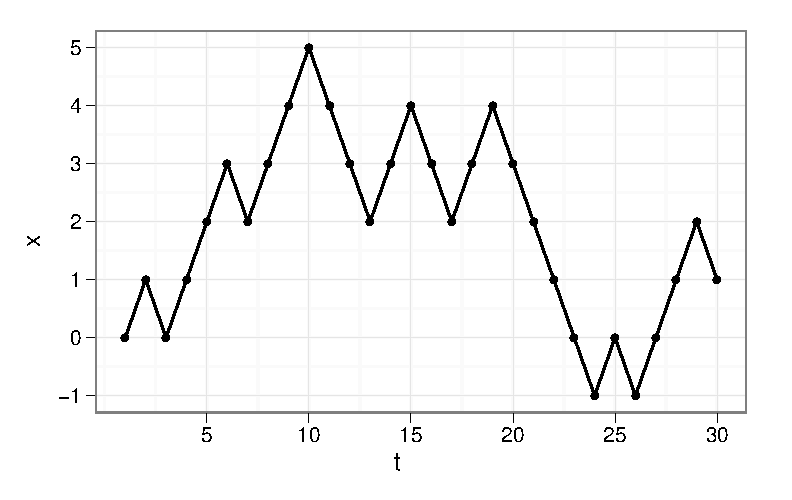
\includegraphics[bb=0 0 380 240, clip, width=300 bp]{random_walk2.pdf}
  \end{center}
  \caption{ランダムウォークの1例}
  \label{random_walk_plot}
\end{figure}

\begin{description}
\item[Monte Carlo] モンテカルロ(法)\\
乱数を用いた計算アルゴリズムを一般にモンテカルロ法と呼ぶ。
名前は,カジノで有名なモンテカルロ(モナコ)から取られた。
\end{description}

そして,MCMCを一言で説明するなら,

\vspace{2zw}
\hspace{10mm}
\begin{minipage}{110mm}
\begin{breakbox}
\noindent
{\large\bf 乱数を用いてマルコフ連鎖を生成し,それにより母数の事後分布を推定する手法}
\end{breakbox}
\end{minipage}
\vspace{2zw}

\noindent
となるだろう。というのも,

\vspace{2zw}
\hspace{10mm}
\begin{minipage}{110mm}
\begin{breakbox}
\noindent
{\large\bf うまく工夫したマルコフ連鎖をつくってやることにより,
事後分布からのサンプルと見なせる
データをとりだすことができる}
\end{breakbox}
\end{minipage}
\vspace{2zw}

\noindent
からである。

%ページ調整
%\vspace{4zw}

\subsection{MCMCのアルゴリズム}

MCMCのアルゴリズムとしては,Metropolis-Hastingsアルゴリズムや,
その特殊な場合にあたるGibbs samplerがよく用いられる。\cite{PRML,Iba2005,Toyoda,Watanabe}
最近は,Hamiltonian Monte Carlo(またはHybrid Monte Carlo)
\cite{PRML,BDA3,Toyoda2015,Watanabe}
を使用したソフトウェアもある。
アルゴリズムについて詳しく知りたい方は参考文献を参照されたい。


\section{MCMCのためのソフトウェア}
CやFortranなどでMCMCのプログラムを作成することも可能だが,
専用のソフトウェアを使う方が簡単であろう。
\begin{itemize}
\item  \textsf{R}上で: MCMCpackなど
\item 専用ソフトウェア: \textsf{WinBUGS}, \textsf{OpenBUGS}, \textsf{JAGS}, \textsf{Stan}など
\begin{itemize}
 \item  上に挙げたもののうち,\textsf{Stan}以外は,BUGS (\textbf{B}ayesian inference \textbf{U}sing
 \textbf{G}ibbs \textbf{S}ampling)言語\cite{BUGSBook, BUGS}という
 モデリング言語を使用している。
 \label{BUGS}
\textsf{Stan}は,BUGSとは異なる言語仕様である。
\item  いずれにも\textsf{R}から使えるようにするパッケージあり
(それぞれ\textsf{R2WinBUGS}, \textsf{R2OpenBUGS}, \textsf{rjags}, \textsf{rstan}など)。
\end{itemize}
\item \textsf{Python}のパッケージもある(\textsf{PyMC}, \textsf{PyStan}など)。
\end{itemize}

\subsection{MCMCpack}

\begin{itemize}
\item ウェブサイト: \texttt{\url{http://mcmcpack.berkeley.edu/}}
\item 最新版: 1.4-0
\item \textsf{R}のパッケージ
\item CRANからインストールできる。
\item Metropolis samplerを使う。
\item \texttt{MCMClogit()},\texttt{MCMCpoisson()}などの関数が用意されており,
これらを使用してMCMC計算ができる。
一部の混合効果モデル(ランダム効果のあるモデル)にも対応している
(\texttt{MCMChregress()},\texttt{MCMChlogit()},
\texttt{MCMChpoisson()}など)。
このように主要なモデルに対応した関数が30個あまりある。
自分で定義した確率分布を使用するときは\texttt{MCMCmetrop1R()}関数を使用する。
参考文献\cite{MCMCpack}に解説あり。
\end{itemize}

\subsection{WinBUGS}

\begin{itemize}
\item ウェブサイト:\\
  \url{http://www.mrc-bsu.cam.ac.uk/software/bugs/the-bugs-project-winbugs/}
\item 最新版: 1.4.3 (開発は終了している)
\item ソースコードは非公開なので,内部のアルゴリズムの確認や,改造はできない。
\item Windows用ソフトだが,\textsf{Wine}\footnote{\url{http://www.winehq.org/} 名前は,
``Wine Is Not Emulator''の略。Windows互換レイヤーソフトで,Windows用ソフトウェ
  ア(すべてというわけではない)をWindowsなしで動作させることができる。
  最新の安定版は2.0.2。}を使用
  することで,OS XやLinux,BSDでも使用することが可能。
\item GUI環境はあるがあまり使いやすくない。\textsf{R2WinBUGS}パッケージ
  で \textsf{R}と連携可能なので,そちらから使う方が使いやすい(と思う)。
\end{itemize}

\subsubsection*{インストール}

ウェブサイトからインストーラーをダウンロード
できる。いずれの環境でも\textsf{WinBUGS}のインストール後には1.4.3パッチをあ
て,``key''をインストールすること。``key''をインストールすることにより,
全機能が使えるようになる。

\paragraph{Windowsへのインストール}

インストーラー(\texttt{WinBUGS14.exe})を起動して,あとは指示に従ってい
けばインストールされる。
ただし,Windows Vistaでは,\texttt{C:{\textbackslash}Program~Files}以下に
インストールすると,アクセス制御の
関係でパッチなどが当てられなくなるので,\texttt{C:{\textbackslash}Program~Files}以外への
インストールが推奨されている
\footnote{\url{http://www.mrc-bsu.cam.ac.uk/software/bugs/the-bugs-project-winbugs/#install}}。
インストーラーは64ビットWindowsには非対応である。

\paragraph{Macへのインストール}

Macでは,\textsf{Wine}を利用して\textsf{WinBUGS}を使うことができる。
macOS用の\textsf{Wine}\footnote{\url{https://wiki.winehq.org/MacOSX}}
を利用するか,\textsf{Homebrew}\footnote{\url{http://brew.sh/}}, \textsf{MacPors}\footnote{\url{http://www.macports.org/}}などの
パッケージ管理システムを利用してインストールするのが簡単であろう。
詳細は,ネット上の資料
\footnote{\url{http://www001.upp.so-net.ne.jp/ito-hi/stat/winbugs.html}\\
\url{http://nhkuma.blogspot.jp/2012/12/macosx106-107winbugswiner2winbugs.html}\\
\url{http://nhkuma.blogspot.jp/2012/12/macosx108-mountain-lion-winbugs-wine.html}}を参照するとよい。


\textsf{Wine}をインストールしたら,
これを使用してWindows用インストーラー
(\texttt{WinBUGS14.exe})を起動
し,\textsf{Wine}環境へ
\textsf{WinBUGS}をインストールする
(デフォルトでは\texttt{\textasciitilde/.wine/drive\_c/Program Files}以下にインストールされる)。


\paragraph{Linuxへのインストール}
\textsf{Wine}を使用する。Ubuntuなどの主要なディストリビューションではパッ
ケージ化されているので,それを利用するのが簡単だろう。
\textsf{Wine}を使用してインストーラー(\texttt{WinBUGS14.exe})を起動
し,\textsf{WinBUGS}をインストールする。

BSDその他UNIXも基本的にはLinuxに準じる。

\subsection{OpenBUGS}

\begin{itemize}
\item ウェブサイト \url{http://www.openbugs.net/}
\item 最新版: 3.2.3
\item オーブンソース(ライセンスはGPL)。しかし開発環境が特
  殊(Black Box Component Builder\footnote{\texttt{http://www.oberon.ch/blackbox.html}}と
  いうものを使用)。
\item WindowsおよびLinuxで動作する。
Macでは\textsf{Wine}により利用可能。
\item \textsf{BRUGS}あるいは\textsf{R2OpenBUGS}により
\textsf{R}との連携が可能\cite{Thomas}。
ともにCRANに収録されている。
\end{itemize}

\subsubsection*{インストール}
\paragraph{Windowsへのインストール}
Windows版インストーラーからインストールできる。64ビットWindowsにもインストールできる。
開発元ではWindows XPと8とで動作確認している。

\paragraph{OS Xへのインストール}
\textsf{WinBUGS}と同様に,\textsf{Wine}を導入して,Windows版をインストールする。

\paragraph{Linuxへのインストール}
Linux用ソースパッケージを展開して,コンパイル・インストールする。

%% JAGS
\subsection{JAGS}

\begin{itemize}

\item ウェブサイト:
  \url{http://mcmc-jags.sourceforge.net/}
  
\item 作者ブログ:
  \url{http://martynplummer.wordpress.com/}  

\item 最新版: 4.3.0

\item オープンソース(ライセンスはGPL)。再配布はもちろん,内部の解析,改
  造なども自由にできる。CおよびC++で書かれていて一般的な開発環境でコンパイル
  可能\footnote{農林水産研究情報総合センターの科学技術計算システムでも自分
  でコンパイルして利用できた。}
  (ただし,BLASやLAPACKといった数値演算ライブラリは必要)。

\item コマンドラインからの操作となるが,\textsf{rjags}や\textsf{R2jags},\textsf{runjags}
といったパッケージを
利用することで,\textsf{R}から使用することも可能。
いずれもCRANに収録されている。

\item \textsf{WinBUGS}で解析できる一部のモデルは解析できない
  \footnote{\url{http://hosho.ees.hokudai.ac.jp/~kubo/ce/JagsMisc.html}}。
 もっとも,\textsf{WinBUGS}よりも柔軟なところもある
  \footnote{\url{http://ito-hi.blog.so-net.ne.jp/2007-02-01-1}}。
  
\item \textsf{OpenBUGS}を実行速度を比較すると,いくつかのモデルではとくに遅いことがあるものの,
平均的にはだいたい同等といったところであると
いう\footnote{\url{http://martynplummer.wordpress.com/2010/09/20/how-fast-is-jags/}}。

\end{itemize}

\subsubsection*{インストール}
WindowsおよびMacにはインストーラーが用意されている。
Linux版主要ディストリビューションにはバイナリパッケージがあるので
それを利用できる。
開発環境があれば,ソースから自分でコンパイルすることも比較的簡単である。
詳細はインストールマニュアルを参照。

%% Stan
\subsection{Stan}
\label{Stan}
\begin{itemize}

\item ウェブサイト:
  \url{http://mc-stan.org/}

\item 最新版: 2.16.0
\item オープンソース(BSDライセンスまたはGPL3)。再配布,内部の解析,改
  造なども自由にできる。
\item \textsf{RStan}という\textsf{R}のパッケージもあり,CRANに収録されている。
また,Pyhtonインターフェイスの\textsf{PyStan}もある。
コマンドラインから実行するものは\textsf{CmdStan}と呼ばれる。
\item Stan $\rightarrow$ C++ $\rightarrow$ ネイティブバイナリ,とコンパイルして実行する。
ネイティブバイナリとして実行されるので,インタプリタ形式と比較して高速である。
\item Mac, Windows, Linuxなどに対応している。
\item Hamiltonian Monte Carlo法\cite{PRML, BDA3, Toyoda2015}を使用し,
通常のMCMCよりも高速に目的分布に収束する。
\item 言語仕様は,BUGSとは異なる。
\end{itemize}

\subsubsection*{インストール}
RStanはCRANからインストール可能。
開発環境(C++など)が必要となる。
詳細はウェブサイトやマニュアルを参照。


%\pagebreak

%%
%% ここから実習
%%
\section{例題}

ここからは,簡単な例題を通してMCMCの使い方をみていきたい。

\subsection{最初のモデル: ポアソン回帰}

%簡単な例題から。
まずは次の例題をMCMCを使って解いてみる。

\vspace{1zw}

\hspace{18mm}
\begin{minipage}{100mm}
\begin{breakbox}
ポアソン分布することがわかっている ある母集団から,\\
\hspace{10mm} $\bm{x} = (3, 1, 4, 3, 3, 6, 4, 1, 6, 4, 
       1, 7, 4, 4, 1, 4, 0, 3, 9, 4)$\\
という標本が得られたとき,その母平均$\lambda$を推定する。
\end{breakbox}
\end{minipage}

\vspace{1zw}

\subsubsection{JAGSによるポアソン回帰}

まずここでは\textsf{R}から,\textsf{JAGS}を使ってポアソン回帰をおこなう。
\textsf{R}スクリプトは,サンプルファイルの\texttt{example1.R}である。
\vspace{1zw}

以下,実行例をボックスの中にしめす。なお,``\texttt{>}''は入力行のプロンプトを,
``\texttt{+}''は,前の行からの継続をそれぞれ示す記号であり,実際には入力不要である。

まずは,データをベクトル\texttt{x}に代入する。
\begin{lstlisting}
> x <- c(3, 2, 4, 3, 3, 6, 4, 1, 6, 4,
+        5, 7, 4, 4, 1, 4, 0, 3, 8, 4)
\end{lstlisting}

実際の解析に入る前に,グラフでデータを確認してみる。
\begin{lstlisting}
> h <- hist(x, right = FALSE,
+           breaks = seq(min(x), max(x) + 1, 1),
+           plot = FALSE)
> barplot(h$counts, names.arg = h$breaks[-length(h$breaks)],
+         las = 1, xlab = "x", ylab = "count")
\end{lstlisting}

平均と分散を確認してみる。
\begin{lstlisting}
> mean(x)
[1] 3.8
> var(x)
[1] 3.957895
\end{lstlisting}

GLMなら以下のようなコードとなる。
\begin{lstlisting}
> fit <- glm(x ~ 1, family = poisson(link = log))
> summary(fit)

Call:
glm(formula = x ~ 1, family = poisson(link = log))

Deviance Residuals: 
    Min       1Q   Median       3Q      Max  
-2.7568  -0.4262   0.1017   0.2230   1.8738  

Coefficients:
            Estimate Std. Error z value Pr(>|z|)    
(Intercept)   1.3350     0.1147   11.64   <2e-16 ***
---
Signif. codes:  0 ‘***’ 0.001 ‘**’ 0.01 ‘*’ 0.05 ‘.’ 0.1 ‘ ’ 1

(Dispersion parameter for poisson family taken to be 1)

    Null deviance: 23.462  on 19  degrees of freedom
Residual deviance: 23.462  on 19  degrees of freedom
AIC: 85.444

Number of Fisher Scoring iterations: 4

> print(exp(coef(fit)))
(Intercept) 
        3.8 
\end{lstlisting}

ではここからいよいよ\textsf{JAGS}による解析を始めよう。

\textsf{JAGS}は,\textsf{BUGS}言語で書かれたモデルのパラメーターをMCMCでベイズ推定する。
ここでは,\textsf{BUGS}言語で書かれたモデルコードは別のファイル(\texttt{example1\_model.txt})になっている。
このファイルの内容は以下のようになっている。
\begin{lstlisting}
model {
  # Likelihood
  for (i in 1:N) {
    X[i] ~ dpois(lambda)
  }

  # Prior
  lambda ~ dunif(0, 1000)
}
\end{lstlisting}
%
GLMでは1行で済んだものが,\textsf{BUGS言語}ではかなり長くなってしまった。
しかし,このような記法により,複雑なモデルも記述することができるのである。

1行目の``\texttt{model\{}''と,9行目の``\texttt{\}}''で囲まれた部分がモデルの定義となる。
まず,3〜5行目が尤度の部分となる。
\texttt{dpois}はポアソン分布であり,\texttt{dpois(lambda)}は,平均\texttt{lambda}の
ポアソン分布ということになる。
\texttt{for}ループの構文で,データ\texttt{X[i]}の添え字\texttt{i}の範囲が
$i \in 1, 2, \dots, N$であることを示している。
そして,\texttt{X}が,平均\texttt{lambda}のポアソン分布に従うことを表している。

8行目で,パラメーター\texttt{lambda}の事前分布を定義している。
\texttt{dunif}は一様分布であり,ここでは,0〜1000という範囲の一様分布を
\texttt{lambda}の事前分布として与えている。
事前分布として与えるべき確率分布があらかじめわからない場合には
このような,幅の広い分布が与えられることが多い。
これを「無情報事前分布(non-informative prior)」や「漠然事前分布(vague prior)」という。
じゅうぶんに幅の広い一様分布のほか,分散の大きい正規分布などもよく用いられる。

このモデルを数式で書くなら以下のようになる。
ポアソン分布の確率質量関数は$f(x)=\lambda^{x}e^{-\lambda}/x!$なので,
パラメーター$\lambda$のもとでデータ$\bm{X}$が得られる
尤度$L(\bm{X}  \mid  \lambda)$は以下の式\ref{likelihood_pois}になる。
\begin{align}
L(\bm{X} \mid \lambda) = \prod_{i = 1}^{N}\frac{\lambda^{X_{i}}e^{-\lambda}}{X_{i}!}
\label{likelihood_pois}
\end{align}

式\ref{likelihood_pois}は,簡単に以下のように書くことも多い。
\begin{align*}
\bm{X} \sim \mathrm{Poisson}(\lambda)
\end{align*}

したがって,このモデルの事後分布は以下のようになる。
\begin{align*}
\Pr(\lambda \mid \bm{X}) &\propto L(\bm{X} \mid \lambda) \mathrm{Pr}(\lambda) \\
L(\bm{X} \mid \lambda) \mathrm{Pr}(\lambda) &=\begin{cases}
 \prod_{i = 1}^{N}\frac{\lambda^{X_{i}}e^{-\lambda}}{X_{i}!} \times 10^{-3} & 0 \leq \lambda  < 10^{3}  \\
 0 & 上以外の場合  \label{posterior} \\
\end{cases}
\end{align*}

ここでまた\textsf{R}のコードに戻ろう。
まずは,\textsf{rjags}パッケージを読み込む。
\begin{lstlisting}
> library(rjags)
 要求されたパッケージ coda をロード中です 
Linked to JAGS 4.3.0
Loaded modules: basemod,bugs
\end{lstlisting}

続いて,初期値を定義する。
これらは省略可能で,その場合には自動的に生成される。
ただし,自動的に生成された値のせいでその後の計算がうまくいかないこともある。
初期値についてはさらに,擬似乱数のタネ(\texttt{.RNG.seed})と
擬似乱数発生アルゴリズム(\texttt{.RNG.name})も明示的に指定するようにしている。
これらも省略可能である。
しかし,パラメータの初期値と擬似乱数を固定しておくことで,再現可能(reproducible),
すなわち同じ計算を繰り返したときに同じ結果が得られるようになる。
\begin{lstlisting}
> inits <- vector("list", 3)
> inits[[1]] <- list(lambda = 1,
+                    .RNG.seed = 1,
+                    .RNG.name = "base::Mersenne-Twister")
\end{lstlisting}
%
要素3のリスト\texttt{inits}をまず作っている。
ここでは1番目の要素のみを使用し,
\texttt{lambda}の初期値は1,乱数のタネは1,乱数生成法は Mersenne-Twisterと指定している。

ここまで準備ができたら,\texttt{jags.mode()}関数でJAGSのモデルオブジェクトを
生成する。
引数として,モデルのファイル名,データ,初期値,マルコフ連鎖の数を与える。
\begin{lstlisting}
> model1 <- jags.model("example1_model.txt",
+                      data = list(X = x, N = length(x)),
+                      inits = inits[[1]], n.chains = 1, n.adapt = 0)
Compiling model graph
   Resolving undeclared variables
   Allocating nodes
Graph information:
   Observed stochastic nodes: 20
   Unobserved stochastic nodes: 1
   Total graph size: 24

Initializing model

\end{lstlisting}
%
引数の\texttt{"example1\_model.txt"}は,BUGS言語でモデルが書かれたファイルの名前である。
\texttt{data}引数は,モデルに渡すデータで,ここではBUGS上の\texttt{X}に\textsf{R}上の\texttt{x}を,
\texttt{N}に\texttt{length(x)}をそれぞれ渡すとしている。
\texttt{inits}引数は初期値であり,先に定義した\texttt{inits[[1]]}を渡している。
\texttt{n.chains}引数はマルコフ連鎖の数である。通常は3〜4とするが,説明のためまずは1としている。
\texttt{n.adapt}引数は,\textsf{JAGS}内部でのMCMC計算のための調整(adaptation)に使われる連鎖の長さを指定する。
ここでは説明のために0としている。

つづいて,\texttt{coda.samples()}関数で,MCMCを実行する。
\begin{lstlisting}
> post1 <- coda.samples(model1, variable.names = "lambda",
+                       n.iter = 50)
NOTE: Stopping adaptation

\end{lstlisting}
%
引数の\texttt{variable.names}で,結果を保存するパラメータを指定する(ここでは\texttt{lambda}のみ)。
\texttt{n.iter}で,マルコフ連鎖の長さを指定する。ここでは50としている。


計算されたマルコフ連鎖の軌跡を表示してみる。
\begin{lstlisting}
> traceplot(post1, col = 1, las = 1)
\end{lstlisting}
%
結果は図\ref{fig:trace1}。

\begin{figure}[hbtp]
  \begin{center}
    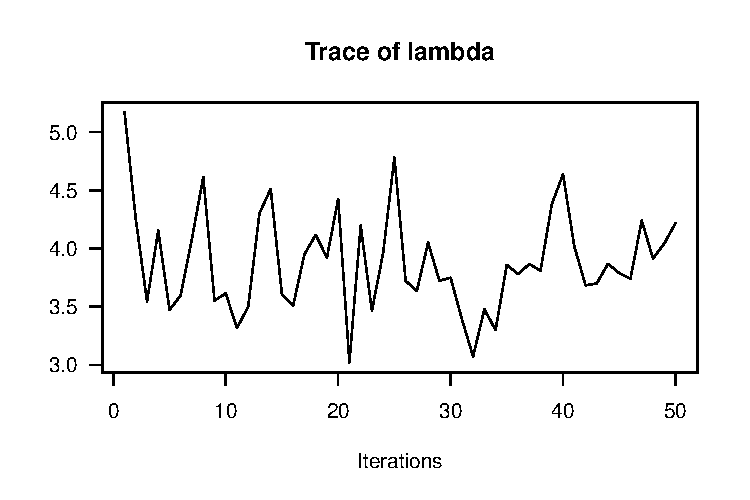
\includegraphics[bb=0 0 360 240, clip, width=240 bp]{example1-1.pdf}
  \end{center}
  \caption{マルコフ連鎖の軌跡}
  \label{fig:trace1}
\end{figure}

別の初期値で試してみよう。
\begin{lstlisting}
> inits[[2]] <- list(lambda = 30,
+                    .RNG.seed = 2,
+                    .RNG.name = "base::Mersenne-Twister")
> inits[[3]] <- list(lambda = 100,
+                    .RNG.seed = 3,
+                    .RNG.name = "base::Mersenne-Twister")
\end{lstlisting}
\texttt{lambda}の初期値は2番目では30,3番目では100としている。
また,乱数のタネは2番目では2,3番目では3としている。

この設定で\textsf{JAGS}を実行する。
\texttt{jags.model()}関数の\texttt{n.chains}引数の値を3としている。
これにより,3本のマルコフ連鎖を使ってパラメーターを推定することになる。
\begin{lstlisting}
> model2 <- jags.model("example1_model.txt",
+                      data = list(X = x, N = length(x)),
+                      inits = inits, n.chains = 3, n.adapt = 0)
Compiling model graph
   Resolving undeclared variables
   Allocating nodes
Graph information:
   Observed stochastic nodes: 20
   Unobserved stochastic nodes: 1
   Total graph size: 24

Initializing model

> post2 <- coda.samples(model2, variable.names = "lambda",
+                       n.iter = 50)
NOTE: Stopping adaptation

\end{lstlisting}

軌跡を表示させる。結果は図\ref{fig:trace3}。
\begin{lstlisting}
> traceplot(post2, las = 1)
\end{lstlisting}

\begin{figure}[hbtp]
  \begin{center}
    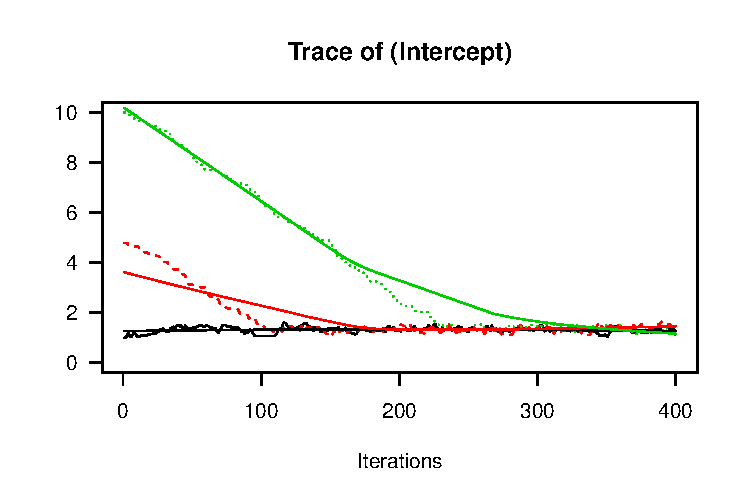
\includegraphics[bb=0 0 360 240, clip, width=260 bp]{example1-2.pdf}
  \end{center}
  \caption{マルコフ連鎖を3つにした結果}
  \label{fig:trace3}
\end{figure}\noindent

初期値により,その影響の残る期間は変わるが,最終的には同じような値に
収束しているように見える。
初期値の影響が残る期間は取り除く必要があり,
この期間のことを,burn-inやwarmupなどと呼ぶ。

では次に,実際に事後分布のサンプルを得ることとする。
設定として,burn-inを1000回(そのうち,500回は\textsf{JAGS}のadaptation),burn-in後の繰り返し回数を1000回,
サンプル取得間隔を1回(つまり毎回)としている。
これらをそれぞれ変数(\texttt{burnin}, \texttt{iter}, \texttt{thin})に代入してから,\texttt{rjags}の関数に渡しているが,もちろん関数の引数に直接数値を渡しても良い。
マルコフ連鎖の数は3としているので,
このとき,取得されるサンプルの大きさは$1000 \div 1 \times 3 = 3000$となる。

\begin{lstlisting}
> burnin <- 1000
> iter <- 1000
> thin <- 1
> model3 <- jags.model("example1_model.txt",
+                      data = list(X = x, N = length(x)),
+                      inits = inits, n.chains = 3, n.adapt = 500)
Compiling model graph
   Resolving undeclared variables
   Allocating nodes
Graph information:
   Observed stochastic nodes: 20
   Unobserved stochastic nodes: 1
   Total graph size: 24

Initializing model

  |++++++++++++++++++++++++++++++++++++++++++++++++++| 100%
> update(model3, n.iter = burnin - 500)
  |**************************************************| 100%
> post3 <- coda.samples(model3,
+                       variable.names = "lambda",
+                       n.iter = iter, thin = thin)
  |**************************************************| 100%
\end{lstlisting}

\texttt{plot()}関数で,マルコフ連鎖の軌跡と事後分布をグラフ表示させる。
結果は図\ref{fig:plot}。
\begin{lstlisting}
> plot(post3)
\end{lstlisting}

\begin{figure}[hbtp]
  \begin{center}
    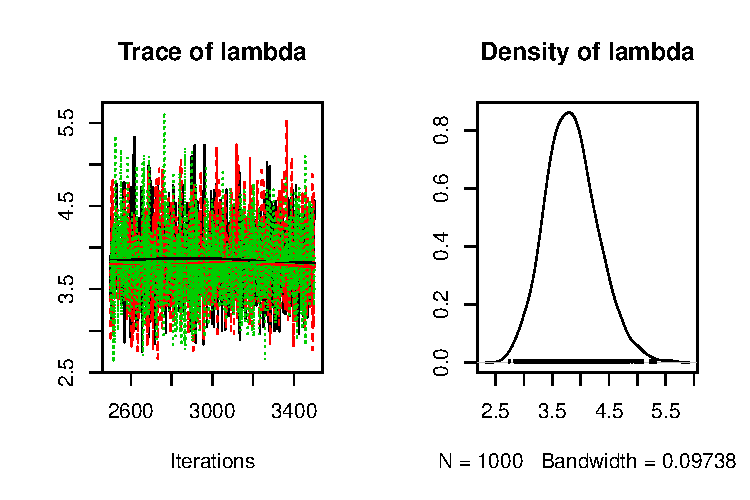
\includegraphics[bb=0 0 360 240, clip, width=260 bp]{example1-3.pdf}
  \end{center}
  \caption{\texttt{plot()}関数の出力結果}
  \label{fig:plot}
\end{figure}\noindent
パラメーター\texttt{lambda}について,各連鎖の軌跡と,全連鎖をまとめた事後分布の密度が図示される。

図\ref{fig:plot}をみると,
3本の連鎖がよく混ざりあっているのがわかる。このように,初期値や擬似乱数系列に
よらず,各連鎖がよく混ざりあっているのは,MCMC計算がうまくいったことを示している。
数値的に収束の診断をおこなう方法は後述する。

\texttt{summary()}関数で結果の要約を表示させる。
\begin{lstlisting}
> summary(post3)

Iterations = 2501:3500
Thinning interval = 1 
Number of chains = 3 
Sample size per chain = 1000 

1. Empirical mean and standard deviation for each variable,
   plus standard error of the mean:

          Mean             SD       Naive SE Time-series SE 
      3.844708       0.460265       0.008403       0.010359 

2. Quantiles for each variable:

 2.5%   25%   50%   75% 97.5% 
3.003 3.524 3.816 4.134 4.807 

\end{lstlisting}
%
ベイズ推定ではパラメーターの推定値も確率的に(事後分布として)与えられる。
その代表値としては一般に平均や中央値が用いられる\footnote{このほか,事後分布のモードを用いる場合もある。これをMAP(Maximum A Posterior)推定値という。}。
また,95\%信用区間\footnote{「頻度主義」統計における信頼区間とは実は違うもの。}も同時に使われることが多い。
この例では,
$\lambda$の事後分布の平均値(事後平均)が3.84,中央値が3.82,95\%信用区間が
3.00〜4.81と推定された。事後平均に対応する$\lambda$の値は$\exp(1.33)=3.78$と
いうことになる。
事後平均・中央値とも,GLMによる最尤推定値とだいたい一致した。

\paragraph{収束診断}
この例ではうまく収束したが,いつでもうまくいくというものでもない。
うまく収束しなかった例を図\ref{bad_mcmc}にしめす。
3本の連鎖がまったく混ざりあっていない。
\begin{figure}[htbp]
	\begin{center}
		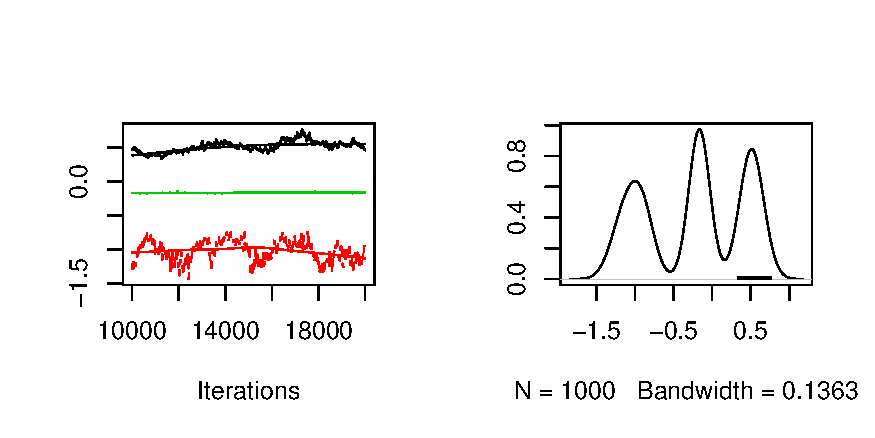
\includegraphics[bb=0 0 420 210, clip, width=320 bp]{bad_mcmc.pdf}
	\end{center}
	\caption{うまく収束しなかった場合}
	\label{bad_mcmc}
\end{figure}

収束状況を数値で診断するためには,Gelman-Rubinの収束診断($\Hat{R}$; Rhat)がよく使われる。
\textsf{R}では,\texttt{coda}パッケージの\texttt{gelman.diag()}関数などで計算できる。
収束していれば$\Hat{R}$の値が1に近くなる(この計算のためには複数の連鎖が必要である)。
詳細は\texttt{help(gelman.diag)}などを参照されたい。
$\Hat{R}$の値は一般には1.1以下でよいとされるが,軌跡とあわせ見て,
収束しているかどうか判断する方がよいだろう。

先に実行したMCMCの結果\texttt{post3}について,$\Hat{R}$を求めてみる。
\begin{lstlisting}
> gelman.diag(post3)
Potential scale reduction factors:

       Point est. Upper C.I.
lambda          1          1

\end{lstlisting}
$\Hat{R}$値は1であった。図\ref{fig:plot}の結果とあわせ,
うまく収束したと言えそうである。

\paragraph{情報事前分布}

次に,情報事前分布を使った例をみてみよう。
今度は,$\lambda$がそれほど大きな値(10以上とか)は取らないだろうと事前の知識で
わかっていたとする。
そこで,$\lambda$の事前分布として$\mathrm{Gamma}(2, 2)$を指定した。
この分布の平均値は1,分散は0.5である。
グラフで示すと,図\ref{prior_posterior}の上の点線のようになる。

\textsf{BUGS}言語によるモデルは以下のようになる。
\begin{lstlisting}
model {
  # Likelihood
  for (i in 1:N) {
    X[i] ~ dpois(lambda)
  }

  # Prior
  lambda ~ dgamma(2, 2)
}
\end{lstlisting}
8行目で,\texttt{lambda}の事前分布にガンマ分布\texttt{dgamma(2, 2)}を使うようになっている。


前の例と同様に,\textsf{JAGS}を実行し,結果を\texttt{post4}に代入する。
%
\begin{lstlisting}
> inits <- list(list(lambda = 0.1,
+                    .RNG.seed = 1,
+                    .RNG.name = "base::Mersenne-Twister"),
+               list(lambda = 1,
+                    .RNG.seed = 2,
+                    .RNG.name = "base::Mersenne-Twister"),
+               list(lambda = 10,
+                    .RNG.seed = 3,
+                    .RNG.name = "base::Mersenne-Twister"))
> model4 <- jags.model("example1-1_model.txt",
+                      data = list(X = x, N = length(x)),
+                      inits = inits, n.chains = 3, n.adapt = 500)
Compiling model graph
   Resolving undeclared variables
   Allocating nodes
Graph information:
   Observed stochastic nodes: 20
   Unobserved stochastic nodes: 1
   Total graph size: 23

Initializing model

> update(model4, n.iter = burnin - 500)
  |**************************************************| 100%
> post4 <- coda.samples(model4,
+                       variable.names = "lambda",
+                       n.iter = iter, thin = thin)
  |**************************************************| 100%
\end{lstlisting}

結果は以下のとおり。無情報事前分布を使用したときの結果よりも,事前分布の
影響を受けて事後平均が小さくなっているのがわかる。

\begin{lstlisting}
> summary(post4)

Iterations = 501:1500
Thinning interval = 1 
Number of chains = 3 
Sample size per chain = 1000 

1. Empirical mean and standard deviation for each variable,
   plus standard error of the mean:

          Mean             SD       Naive SE Time-series SE 
      3.544598       0.396085       0.007231       0.007348 

2. Quantiles for each variable:

 2.5%   25%   50%   75% 97.5% 
2.814 3.272 3.527 3.806 4.378 

\end{lstlisting}

図\ref{prior_posterior}は,事前分布(上の点線)が尤度(下の実線)で更新されて
事後分布(上の実線)となることを示している。

\begin{figure}[htbp]
	\begin{center}
		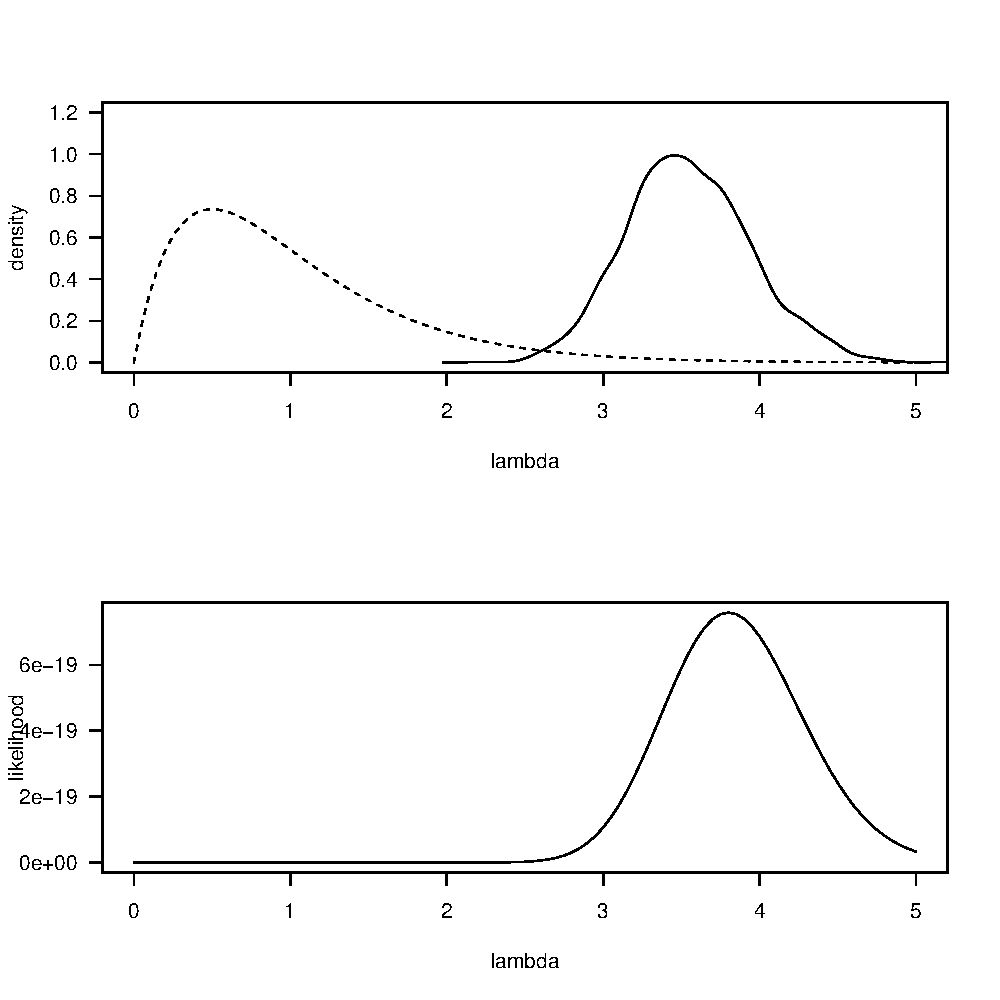
\includegraphics[bb=0 0 480 480, clip, width=320 bp]{example1-4.pdf}
	\end{center}
	\caption{$\lambda$の事前分布(上の点線)・事後分布(上の実線)と,尤度(下)}
	\label{prior_posterior}
\end{figure}


%ページ調整
%\pagebreak

\clearpage

%%
%% ロジスティック回帰
%%
\subsection{ロジスティック回帰}
\label{logistic}


つぎに,以下の問題をMCMCを使用して解いてみる。
\vspace{1zw}

\hspace{18mm}
\begin{minipage}{100mm}
\begin{breakbox}
\noindent
ある生物の集団があったとする。
ある薬品がその生物に及ぼす効果を調べるために,
$N$(=11)段階($\bm{x} = (0, 1, 2, 3, 4, 5, 6, 7, 8, 9, 10)$単位)に薬品の量を変えて
その生物への投与試験をおこなった。
それぞれの量を$K$(=10)個体ずつに
与えたところ,その量$\bm{x}$に応じて
10個体中$\bm{y} = (1, 2, 2, 6, 4, 5, 8, 9, 9, 9, 10)$個体が死亡したとする。
このとき,$\bm{x}$と$\bm{y}$との関係をモデル化し,パラメーターを推定する。
\end{breakbox}
\end{minipage}
\vspace{1zw}

$\bm{x}$と$\bm{y}$との関係をプロットしてみると,図\ref{example2_plot}の
ようになる。

\begin{figure}[htbp]
  \begin{center}
    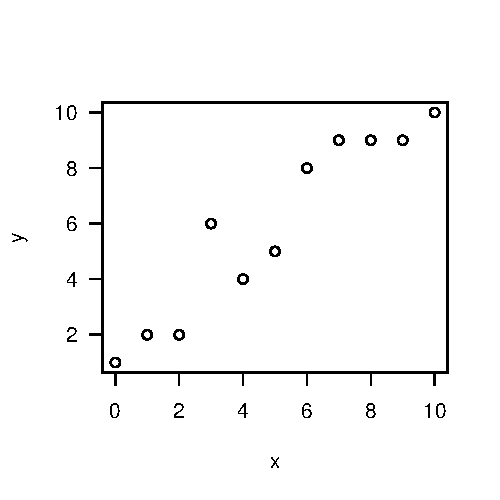
\includegraphics[bb=0 0 240 240, clip, width=160 bp]{example2.pdf}
  \end{center}
  \caption{\ref{logistic}で使用するデータ}
  \label{example2_plot}
\end{figure}

\subsubsection{JAGSによる例}

まず,\textsf{JAGS}でこのデータを解析してみる。
この例題で使用する\textsf{R}スクリプトは\texttt{example2.R},\textsf{BUGS}言語によるモデルは\texttt{example2\_model.txt}である。

\paragraph{データ}
\textsf{R}上で下のようにデータを用意する。
\begin{lstlisting}
> k <- 10
> x <- c(0, 1, 2, 3, 4, 5, 6, 7, 8, 9, 10)
> y <- c(1, 2, 2, 6, 4, 5, 8, 9, 9, 9, 10)
> n <- length(x)
\end{lstlisting}

%ページ調整
%\pagebreak

\paragraph{モデル}
BUGS言語によるモデルは以下のとおり。

\begin{lstlisting}
model {
  # Likelihood
  for (i in 1:N) {
    logit(p[i]) <- beta + beta.x * X[i]
    Y[i] ~ dbin(p[i], K)
  }

  # Priors
  beta ~ dnorm(0, 1.0E-4)
  beta.x ~ dnorm(0, 1.0E-4)
}
\end{lstlisting}

では,このモデルについて詳しくみてみよう。
3行目から6行目が尤度の部分である。
\texttt{for}ループの構文で,\texttt{for}ブロック内の式の変数\texttt{X[i]}, \texttt{Y[i]}, 
\texttt{p[i]}の\texttt{i}の範囲が
$i \in 1, 2, \dots, N$であることを示している。
\texttt{dbin(p, n)}は二項分布$\mathrm{Binomial}(n, p)$
(\texttt{p}は確率。\texttt{n}は試行回数)。
``\texttt{\textasciitilde}''(チルダ)は,左辺の変数が右辺の確率分布に従うことをしめす。
\texttt{logit(p)}はロジット関数
$\mathrm{logit}(p) = \log(p/(1-p))$
である。
ここでは,\texttt{Y}が,試行回数\texttt{K}および確率\texttt{p}の二項分布に
従い,\texttt{p}のロジットが\texttt{X}と線形の関係にあるとモデル化している。

つぎに,9行目から10行目で\texttt{beta}および\texttt{beta.x}の事前分布を定義している。
ここでは,
\texttt{beta}および\texttt{beta.x}の事前分布を,$\mathrm{Normal}(0, 10^{4})$,
すなわち平均0,分散が$10^{4}$という確率分布にしている
(BUGS言語の確率分布\texttt{dnorm()}の第1引数は平均,第2引数は精度(分散の逆数))。
これはつまり,無情報事前分布である。
なお,確率的関係(``\texttt{\textasciitilde}'')と決定論的関係(``\texttt{<-}'')の違いに注意すること。

以上を数式で表現すると以下のようになる。
\begin{align*}
\Pr(\beta, \beta_x|\bm{X}, \bm{Y}) &\propto L(\bm{X}, \bm{Y}|\beta, \beta_x)\Pr(\beta)\Pr(\beta_x) \\
L(\bm{X}, \bm{Y}|\beta, \beta_x) &= \prod_{i=1}^{N}{\mathrm{Binomial}(Y_i|K, p(X_i))} \notag \\
  &= \prod_{i=1}^{N}{\frac{K!}{Y_i!(K-Y_i)!}p(X_i)^{Y_i}(1-p(X_i))^{K-Y_i}}
\intertext{ただし,}
p(X_i) &= \mathrm{logit}^{-1}(\beta+\beta_{x}X_i)) \notag \\
  &= \frac{\exp(\beta+\beta_{x}X_i)}{1 + \exp(\beta+\beta_{x}X_i)} \\
\Pr(\beta) &= \mathrm{Normal}(0, 10^{6}) \\
\Pr(\beta_{x}) &= \mathrm{Normal}(0, 10^{6})
\end{align*}

\paragraph{設定}

つづいて,マルコフ連鎖の数,パラメーターの初期値を決める。
\begin{lstlisting}
> ## Number of chains
> n.chains <- 3
> 
> ## Initial values
> inits <- vector("list", n.chains)
> inits[[1]] <- list(beta = -10, beta.x = 0,
+                    .RNG.seed = 314,
+                    .RNG.name = "base::Mersenne-Twister")
> inits[[2]] <- list(beta =  -5, beta.x = 2,
+                    .RNG.seed = 3141,
+                    .RNG.name = "base::Mersenne-Twister")
> inits[[3]] <- list(beta =   0, beta.x = 4,
+                    .RNG.seed = 31415,
+                    .RNG.name = "base::Mersenne-Twister")
> 
> ## Model file
> model.file <- "example2_model.txt"
> 
> ## Parameters
> pars <- c("beta", "beta.x")
\end{lstlisting}
%
ここでは,マルコフ連鎖の数を3とし,
\texttt{beta}と\texttt{beta.x}とについてそれぞれの連鎖について初期値を
定義している。

また,モデルのファイル名(\texttt{model.file})と,
推定結果を保存するパラメーター名(\texttt{pars})もそれぞれ同様に変数に入れている。
後者では,\texttt{beta}と\texttt{beta.x}を指定している。

\paragraph{実行}

ここまで準備ができたら,\texttt{jags.mode()}関数でJAGSのモデルオブジェクトを
生成する。
\begin{lstlisting}
> model <- jags.model(file = model.file,
+                     data = list(N = n, K = k,
+                                 X = x, Y = y),
+                     inits = inits, n.chains = n.chains,
+                     n.adapt = 1000)
  |++++++++++++++++++++++++++++++++++++++++++++++++++| 100%
\end{lstlisting}

続いて,\texttt{update()}関数によりさらにburn-inをおこなう。
\begin{lstlisting}
> update(model, n.iter = 1000)
  |**************************************************| 100%
\end{lstlisting}

そして,\texttt{coda.samples()}関数によりMCMCのサンプルを得る。
各連鎖について,繰り返し回数3000回,サンプリング間隔3回としている。

\begin{lstlisting}
> post <- coda.samples(model, n.iter = 4000, thin = 4,
+                      variable.names = pars)
  |**************************************************| 100%
\end{lstlisting}


\paragraph{結果表示}

結果をプロットしてみる(図\ref{plot_coda})。
\begin{lstlisting}
> plot(post)
\end{lstlisting}


\begin{figure}[htbp]
	\begin{center}
		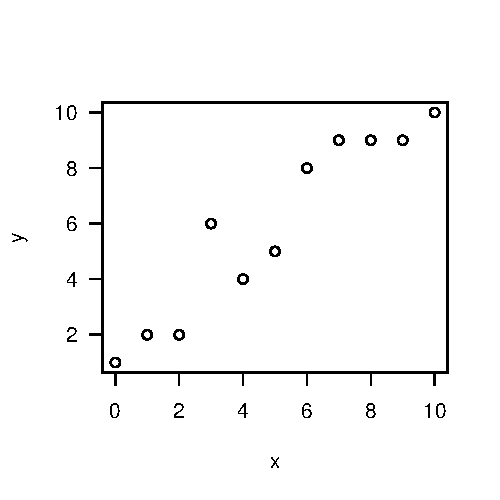
\includegraphics[bb=0 0 400 400, clip, width=300 bp]{example2.pdf}
	\end{center}
	\caption{例題2のMCMC計算の結果}
	\label{plot_coda}
\end{figure}


\texttt{gelman.diag()}関数でGelman-Rubin統計量($\Hat{R}$)を表示させてみると,
両パラメーターについて1に近い値となっており,
図\ref{plot_coda}の軌跡とあわせて,うまく収束したことが
確認できる。
\begin{lstlisting}
> gelman.diag(post)
Potential scale reduction factors:

       Point est. Upper C.I.
beta         1.01       1.02
beta.x       1.00       1.01

Multivariate psrf

1.01
\end{lstlisting}

%ページ調整
%\pagebreak

結果の要約を表示する。
\begin{lstlisting}
> summary(post)

Iterations = 2004:6000
Thinning interval = 4 
Number of chains = 3 
Sample size per chain = 1000 

1. Empirical mean and standard deviation for each variable,
   plus standard error of the mean:

          Mean     SD Naive SE Time-series SE
beta   -2.1802 0.4960 0.009055       0.014823
beta.x  0.5609 0.1021 0.001864       0.003053

2. Quantiles for each variable:

          2.5%     25%    50%     75%   97.5%
beta   -3.1821 -2.5045 -2.160 -1.8401 -1.2539
beta.x  0.3762  0.4914  0.554  0.6248  0.7721

\end{lstlisting}

\noindent
\texttt{beta}の事後平均が-2.18,95\%信用区間が-3.18〜-1.25,
\texttt{beta.x}の事後平均が0.56,95\%信用区間が0.38〜0.77
と推定された。

%ページ調整
%\vspace{1zw}

つづいて,$\bm{X}$と$\bm{Y}$とのプロットに,$\bm{Y}$の期待値を重ねて表示させてみよう。
\begin{lstlisting}
> beta <- unlist(post[, "beta"])
> beta.x <- unlist(post[, "beta.x"])
> 
> new.x <- seq(0, 10, len = 100)
> logit.p <- beta + beta.x %o% new.x
> exp.y <- k * exp(logit.p) / (1 + exp(logit.p))
> y.mean <- apply(exp.y, 2, mean)
> y.975 <- apply(exp.y, 2, quantile, probs = 0.975)
> y.025 <- apply(exp.y, 2, quantile, probs = 0.025)
> y.995 <- apply(exp.y, 2, quantile, probs = 0.995)
> y.005 <- apply(exp.y, 2, quantile, probs = 0.005)
> 
> plot(x, y, type = "p", ylim = c(0, 10), las = 1)
> lines(new.x, y.mean, lty = 1)
> lines(new.x, y.975, lty = 2)
> lines(new.x, y.025, lty = 2)
> lines(new.x, y.995, lty = 3)
> lines(new.x, y.005, lty = 3)
> legend("bottomright",
+        legend = c("mean", "95% interval", "99% interval"),
+        lty = c(1, 2, 3))
\end{lstlisting}
\noindent
\texttt{post}には,各連鎖をリストの要素として,
各パラメーターについて
サンプリングされた値が格納されているので,それを取り出して使っている。
1行目と2行目の\texttt{unlist()}関数は,リスト構造になっているものを
まとめて単純なベクトルとする関数である。

Xの値をすこしづつ変えながら,MCMCでサンプリングされたすべての値についてYの値を
計算して,その期待値および信用区間を計算させている。
表示結果は図\ref{example2exp_plot}。
\begin{figure}[htbp]
  \begin{center}
    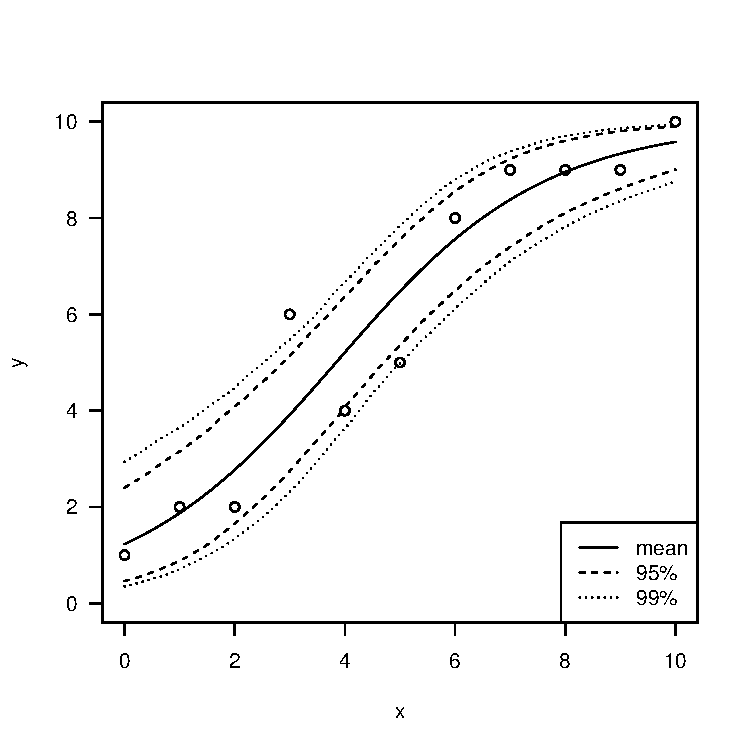
\includegraphics[bb=0 0 360 360, clip, width=240 bp]{example2_exp.pdf}
  \end{center}
  \caption{\ref{logistic}で使用したデータ(点)とYの期待値および信用区間(曲線)}
  \label{example2exp_plot}
\end{figure}

%ページ調整
%\pagebreak

\subsubsection{Stanによる例}
同じ問題を\textsf{Stan}により解いてみる。
\textsf{R}スクリプトは\texttt{example2\_Stan.R}である。
RStanを使用する。
%
\begin{lstlisting}
> library(rstan)
\end{lstlisting}

モデルの定義。
ここでは,\texttt{example2.stan}というファイルでモデルを記述している。
%
\begin{lstlisting}
data {
  int<lower = 0> N;
  int<lower = 0> K;
  vector[N] X;
  int<lower = 0, upper = 10> Y[N];
}

parameters {
  real beta;
  real beta_x;
}

transformed parameters {
  vector[N] logit_p;

  logit_p = beta + beta_x * X;
}

model {
  // Likelihood
  Y ~ binomial_logit(K, logit_p);

  // Priors
  beta ~ normal(0.0, 1.0e+3);
  beta_x ~ normal(0.0, 1.0e+3);
}
\end{lstlisting}
\noindent
Stanのモデルの記述は,\texttt{data},\texttt{parameters},
\texttt{transformed parameters},\texttt{model}などのブロックからなる
(詳細はマニュアルを参照)。
また,データや推定するパラメーターには型の宣言が必要である。この際,
とりうる値の上限・下限を設定することもできる。
なお,変数名などに``\texttt{.}''(ピリオド)は使用できない。
かわりに``\texttt{\_}''(アンダーバー)を使うようにする。
また,行末には必ずセミコロン(;)をつける。
%Stan 2.10からは,代入には``\texttt{<-}''ではなく``\texttt{=}''を使用することが推奨されるようになった。

21行目の\texttt{binomial\_logit}分布は,logitスケール($-\infty$〜$\infty$)のパラメーターを引数にとる2項分布である。
ここで使用するパラメーター\texttt{logit\_p}は,\texttt{transformed parameters}ブロック中の16行目で
定義されている。

\textsf{R}コードで,連鎖の数,初期値,保存するパラメーターを設定する。
\begin{lstlisting}
> n.chains <- 3
> inits <- vector("list", 3)
> inits[[1]] <- list(beta = -10, beta_x = 0)
> inits[[2]] <- list(beta =  -5, beta_x = 2)
> inits[[3]] <- list(beta =   0, beta_x = -2)
> pars <- c("beta", "beta_x")
\end{lstlisting}

\texttt{stan()}関数によりStanを実行して,結果を\texttt{fit}というオブジェクトに格納する。
\begin{lstlisting}
> fit <- stan(model_code = example2_code,
+             data = list(X = x, Y = y, N = n, K = k),
+             pars = pars, init = inits, seed = 123,
+             chains = n.chains,
+             iter = 2500, warmup = 500, thin = 2)
\end{lstlisting}
\noindent
\texttt{warmup}はburn-inとおなじものと思ってよい(細かな相違点は参考文献\cite{BDA3}を参照)。

結果を表示する。
\begin{lstlisting}[basicstyle=\ttfamily\footnotesize]
> print(fit)
Inference for Stan model: example2.
3 chains, each with iter=2500; warmup=500; thin=2; 
post-warmup draws per chain=1000, total post-warmup draws=3000.

         mean se_mean   sd   2.5%    25%    50%    75%  97.5% n_eff Rhat
beta    -2.19    0.01 0.51  -3.22  -2.51  -2.17  -1.85  -1.23  1287    1
beta_x   0.56    0.00 0.10   0.37   0.49   0.56   0.63   0.78  1144    1
lp__   -51.93    0.03 1.03 -54.66 -52.33 -51.60 -51.20 -50.93  1406    1

Samples were drawn using NUTS(diag_e) at Mon Aug 14 10:04:01 2017.
For each parameter, n_eff is a crude measure of effective sample size,
and Rhat is the potential scale reduction factor on split chains (at 
convergence, Rhat=1).
\end{lstlisting}
\noindent
なお,\texttt{lp\_\_}はモデルの対数確率である。

\subsubsection{うまくいかないとき}
MCMC計算がうまくいかないときは,まず \textsf{R}コードおよびモデルコード,初期値,データ
をよく見直そう。

\paragraph{エラーになるとき}
エラーが発生してMCMC計算が途中で(あるいは最初から)止まってしまうときは,
まずはエラーメッセージを確認してみる。
とくに\textsf{WinBUGS}や\textsf{OpenBUGS}では,
どこでエラーになっているのか わかりづらいこともままあるが,
下のような点を確認してみる。
\begin{itemize}
\item 構文に誤りはないか? 
\begin{itemize}
\item ``\texttt{\textasciitilde}''と``\texttt{<-}''とを間違えていないか?
\item カッコ(``\texttt{()}''や``\texttt{\{\}}'')の対応はあっているか?
\end{itemize}
\item 変数名などにtypoがないか?
\item 配列の次数や,添字の範囲は正しいか?
\item 初期値がおかしくないか?
\begin{itemize}
\item 例: ガンマ分布なのに負の値を与えている。
\item 数値的にあり得ない値というわけでなくても,あまり極端な値だとエラーが発生することがある。
\end{itemize}
\item モデルに誤りがないか?
\begin{itemize}
\item 事前分布の定義漏れはないか。また逆に,2重定義はされていないか。
\item 確率分布の引数に与える値は,その確率分布にあっているか。
\begin{itemize}
\item 例: ポアソン分布の平均として与える値に負の値が発生している。
\end{itemize}
\end{itemize}
\end{itemize}

\paragraph{MCMC計算が収束しないとき}
エラーは発生しないものの,MCMC計算が収束しないときは下のような点に気をつけてみる。
\begin{itemize}
\item モデルを見直す。
\begin{itemize}
\item データと確率分布があっているか?
\item モデルが必要以上に複雑でないか?
\item 余分なパラメーターがないか?
\end{itemize}
\item マルコフ連鎖の長さを長くして,サンプリング間隔を長くする。
  ただし必然的に計算時間は長くなる。モデルの改良のような本質的な
  改善ではないが,もう少し収束をよくしたいというようなときには
  有効なこともある。
\end{itemize}

%ページ調整
%\pagebreak

\subsection{線形混合モデル,あるいは階層ベイズモデル}
\label{mixed_model}

以下の問題を考える。
\vspace{1zw}

\hspace{18mm}
\begin{minipage}{100mm}
\begin{breakbox}
\noindent
ある調査を,全体を8つのブロックに分けておこない,
各ブロックごとに5組の観察データを
3つの変量($X_1,$ $X_2$, $Y$)について集めた。
変量$Y$は,$X_1$と$X_2$とに影響を受けており,その関係は線形であるとする。
これをモデル化して,パラメーターの推定をおこなう。
このとき,回帰したときの切片にブロックごとに多少の上下(ランダム効果,
あるいは変量効果)があることを想定する。
\end{breakbox}
\end{minipage}

\vspace{1zw}

\paragraph{データ}
今回のデータはあらかじめファイルに保存してある。``\texttt{example3.csv}''から読み込む。
\begin{lstlisting}
> data <- read.csv("example3.csv")
\end{lstlisting}


最初の10行の内容を表示してみると,以下のとおり。
%\vspace{0.5em}
\begin{lstlisting}
> head(data, 10)
   block   x1   x2    y
1      1 5.56 1.64 5.13
2      1 5.13 2.40 4.53
3      1 4.89 3.83 4.37
4      1 5.61 3.92 4.18
5      1 5.01 4.59 2.80
6      2 4.72 3.51 3.14
7      2 4.86 3.13 1.87
8      2 5.86 5.30 4.67
9      2 4.97 3.14 3.60
10     2 4.26 3.29 1.73
\end{lstlisting}

散布図行列を表示して,データを確認する。結果は図\ref{example3_pairs_plot}。

%\vspace{0.5em}
\begin{lstlisting}
> pairs(data)
\end{lstlisting}
%\vspace{0.5em}

\begin{figure}[htbp]
	\begin{center}
		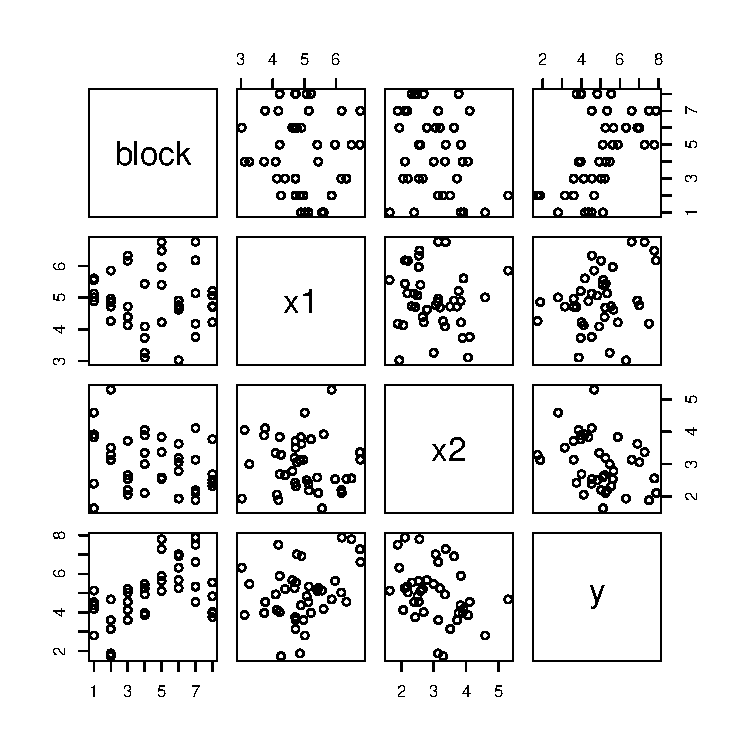
\includegraphics[bb=0 0 360 360, clip, width=270 bp]{example3_pairs.pdf}
	\end{center}
	\caption{\ref{mixed_model}で使用するデータ}
	\label{example3_pairs_plot}
\end{figure}

\textsf{JAGS}を使用してパラメーター推定をおこなうこととする。
使用する\textsf{R}スクリプトは``\texttt{example3.R}''である。

%ページ調整
%\vspace{3zw}

まず,データを行列の形に変換する(BUGSのモデルで使用する形式にあわせるため)。
各行が,各ブロックのデータとなる。

\begin{lstlisting}
> n.block <- max(data$block)      # number of blocks
> n.data <- nrow(data) / n.block  # number of data in a block
>
> x1 <- t(matrix(data$x1, nrow = n.data, ncol = n.block))
> x2 <- t(matrix(data$x2, nrow = n.data, ncol = n.block))
> y  <- t(matrix(data$y,  nrow = n.data, ncol = n.block))
\end{lstlisting}

%ページ調整
%\vspace{3zw}


\texttt{x1}の内容を確認する。
\begin{lstlisting}
> print(x1)
     [,1] [,2] [,3] [,4] [,5]
[1,] 5.56 5.13 4.89 5.61 5.01
[2,] 4.72 4.86 5.86 4.97 4.26
[3,] 4.13 4.72 4.39 6.33 6.17
[4,] 5.44 3.26 3.73 3.11 4.09
[5,] 5.41 6.49 6.76 5.97 4.22
[6,] 3.02 4.76 4.91 4.69 4.62
[7,] 6.77 3.76 4.18 5.14 6.18
[8,] 4.73 4.71 5.07 5.21 4.22
\end{lstlisting}

\paragraph{モデル}
ブロックをランダム効果としてモデルに組み込む。
$\epsilon_{\mathrm{B}i}$をブロック$i$のランダム効果の値とし,
$\sigma_\mathrm{B}$をその事前分布の標準偏差とする。
\begin{align*}
Y_{ij} &\sim \mathrm{Normal}(\mu_{ij}, \sigma^{2}) \\
\mu_{ij} &= \beta + \beta_{1} X_{1ij} + \beta_{2} X_{2ij} + \epsilon_{\mathrm{B}i} \\
\epsilon_{\mathrm{B}i} &\sim \mathrm{Normal}(0, \sigma_\mathrm{B}^{2})
\end{align*}
\noindent
ここで,$\mu_{ij}$はブロック$i$の$j$番目の観測値の期待値,$\sigma$はその標準偏差である。
$\beta$は線形モデル部分の切片,$\beta_{1}$,$\beta_{2}$はそれぞれ$X_{1}$,$X_{2}$の
係数である。

このモデルをBUGS言語で記述すると以下のようになる。
このモデルを,``\texttt{example3\_model.txt}''というファイル名で保存しておく。

\begin{lstlisting}
var
  M,                    # Number of blocks
  N,                    # Number of observations per block
  X1[M, N], X2[M, N],   # Data
  Y[M, N],
  e.B[M],               # Random effect
  beta, beta.1, beta.2, # Parameters
  tau, sigma, 
  tau.B, sigma.B;       # Hyperparameters

model {
  # Likelihood
  for (i in 1:M) {
    for (j in 1:N) {
      Y[i, j] ~ dnorm(mu[i, j], tau)
      mu[i, j] <- beta + beta.1 * X1[i, j] +
                         beta.2 * X2[i, j] + e.B[i]
    }
    e.B[i] ~ dnorm(0, tau.B)
  }

  # Priors
  beta ~ dnorm(0, 1.0E-4)
  beta.1 ~ dnorm(0, 1.0E-4)
  beta.2 ~ dnorm(0, 1.0E-4)
  tau <- 1 / (sigma * sigma)
  tau.B <- 1 / (sigma.B * sigma.B)
  sigma ~ dunif(0, 1.0E+4)
  sigma.B ~ dunif(0, 1.0E+4)
}
\end{lstlisting}

BUGS言語では,変数宣言は必ずしも必要ではないが,高次元配列については
変数宣言が必要となる場合がある。
その場合も,通常のパラメーターの変数などは宣言しなくてもよいが,宣言して
おいたほうがコードの可読性がよくなる(と思う)ので今回は
宣言してある。

このモデルでは,
ブロックによるランダム効果\texttt{e.B[]}の事前分布は,平均が0,分散が1/\texttt{tau.B}
($\texttt{tau.B}=1/\texttt{sigma.B}^{2}$)の
正規分布としている(18行目)。
また,\texttt{sigma.B}の事前分布は[0, 10000]の一様分布としている(28行目)。
すなわちここでは,\texttt{tau.B}(\texttt{sigma.B})が,
パラメーター\texttt{e.B[]}の事前分布を決める
超パラメーター(hyperparameter)となっている(図\ref{example3_schema})。
このようにパラメーターが階層化されているモデルを「階層ベイズモデル」と呼ぶ。

\begin{figure}[htbp]
	\begin{center}
		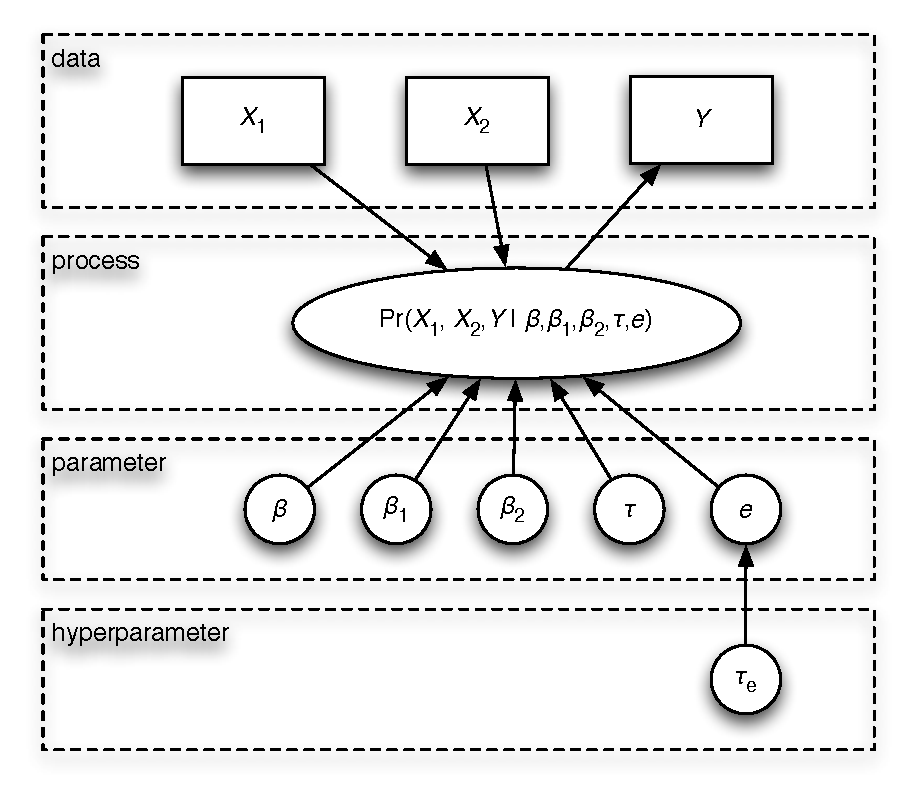
\includegraphics[bb=0 0 440 384, clip, width=280 bp]{example3_schema.pdf}
	\end{center}
	\caption{モデルの概念図}
	\label{example3_schema}
\end{figure}

%ページ調整
%\pagebreak

\paragraph{実行}

前の節と同様に,\textsf{rjags}を使って実行する。
このモデルの場合,\textsf{JAGS}の\texttt{bugs}モジュールを読み込んでおくと
収束が速い(2行目)。

\begin{lstlisting}
> library(rjags)
> load.module("glm")
>
> ## Model file
> model.file <- "example3_model.txt"
> 
> ## Number of chains
> n.chains <- 3
> 
> ## Initial values
> inits <- vector("list", n.chains)
> inits[[1]] <- list(beta =  5, beta.1 = 0, beta.2 = 0,
+                    sigma = 1, sigma.B = 1,
+                    .RNG.seed = 123,
+                    .RNG.name = "base::Mersenne-Twister")
> inits[[2]] <- list(beta =  -5, beta.1 = 10,  beta.2 = 10,
+                    sigma = 10, sigma.B = 10,
+                    .RNG.seed = 1234,
+                    .RNG.name = "base::Mersenne-Twister")
> inits[[3]] <- list(beta = 0, beta.1 = -10,  beta.2 = -10,
+                    sigma = 5, sigma.B = 5,
+                    .RNG.seed = 12345,
+                    .RNG.name = "base::Mersenne-Twister")
> 
> ## Parameters
> pars <- c("beta", "beta.1", "beta.2",
+           "sigma", "sigma.B", "e.B")
> 
> ## MCMC
> model <- jags.model(file = model.file,
+                     data = list(M = n.block, N = n.data,
+                                 X1 = x1, X2 = x2, Y = y),
+                     inits = inits, n.chains = n.chains,
+                     n.adapt = 1000)
  |++++++++++++++++++++++++++++++++++++++++++++++++++| 100%
>
> ## Burn-in
> update(model, n.iter = 1000)
  |**************************************************| 100%
> 
> ## Sampling
> post <- coda.samples(model, n.iter = 5000, thin = 5,
+                      variable.names = pars)
  |**************************************************| 100%
\end{lstlisting}

\paragraph{結果}

結果は以下のようになる。
%ページ調整
\vspace{1zw}
\begin{lstlisting}
> gelman.diag(post)
Potential scale reduction factors:

        Point est. Upper C.I.
beta          1.00       1.00
beta.1        1.00       1.00
beta.2        1.00       1.00
e.B[1]        1.00       1.01
e.B[2]        1.00       1.01
e.B[3]        1.00       1.00
e.B[4]        1.00       1.00
e.B[5]        1.00       1.00
e.B[6]        1.00       1.00
e.B[7]        1.00       1.00
e.B[8]        1.00       1.00
sigma         1.00       1.01
sigma.B       1.01       1.01

Multivariate psrf

1.01
> summary(post)

Iterations = 2005:7000
Thinning interval = 5 
Number of chains = 3 
Sample size per chain = 1000 

1. Empirical mean and standard deviation for each variable,
   plus standard error of the mean:

           Mean     SD Naive SE Time-series SE
beta     3.6686 1.2531 0.022879       0.021932
beta.1   0.4730 0.1893 0.003456       0.003420
beta.2  -0.3347 0.2041 0.003727       0.003790
e.B[1]  -0.7469 0.6344 0.011582       0.010847
e.B[2]  -1.5685 0.6465 0.011804       0.011794
e.B[3]  -0.6384 0.6239 0.011391       0.011331
e.B[4]   0.2383 0.6463 0.011800       0.011798
e.B[5]   0.8257 0.6324 0.011545       0.011547
e.B[6]   1.2837 0.6373 0.011635       0.011635
e.B[7]   1.0147 0.6262 0.011432       0.011089
e.B[8]  -0.5320 0.6321 0.011541       0.011544
sigma    0.9220 0.1232 0.002249       0.002386
sigma.B  1.3421 0.5206 0.009505       0.010773

2. Quantiles for each variable:

           2.5%     25%     50%     75%    97.5%
beta     1.2390  2.8462  3.6457  4.4993  6.13027
beta.1   0.1037  0.3445  0.4744  0.5941  0.85960
beta.2  -0.7474 -0.4635 -0.3318 -0.2021  0.07519
e.B[1]  -2.0262 -1.1427 -0.7286 -0.3519  0.49027
e.B[2]  -2.8444 -1.9895 -1.5580 -1.1774 -0.34317
e.B[3]  -1.8713 -1.0220 -0.6391 -0.2360  0.57344
e.B[4]  -1.0221 -0.1700  0.2313  0.6367  1.54991
e.B[5]  -0.3757  0.4150  0.8265  1.2236  2.09405
e.B[6]   0.1185  0.8862  1.2606  1.6786  2.58318
e.B[7]  -0.1809  0.5955  1.0096  1.3959  2.27913
e.B[8]  -1.8475 -0.9065 -0.5262 -0.1399  0.68231
sigma    0.7218  0.8342  0.9092  0.9956  1.20375
sigma.B  0.6712  0.9938  1.2313  1.5683  2.65059

\end{lstlisting}

\texttt{e.B[]}の事後分布は図\ref{example3_e_plot}のようになっている。

%%\begin{breakbox}
%\begin{verbatim}
%plot(NULL, type = "n",
%     xlim = c(-2, 2), ylim = c(0, 2.5),
%     xlab = "value", ylab = "density",
%     main = "Posterior destribution of e[]",
%     las = 1)
%for (i in 1:n.block) {
%  lines(density(post.samp$sims.list$e[,i]), col = i)
%}
%\end{verbatim}
%\end{breakbox}

\begin{figure}[htbp]
	\begin{center}
		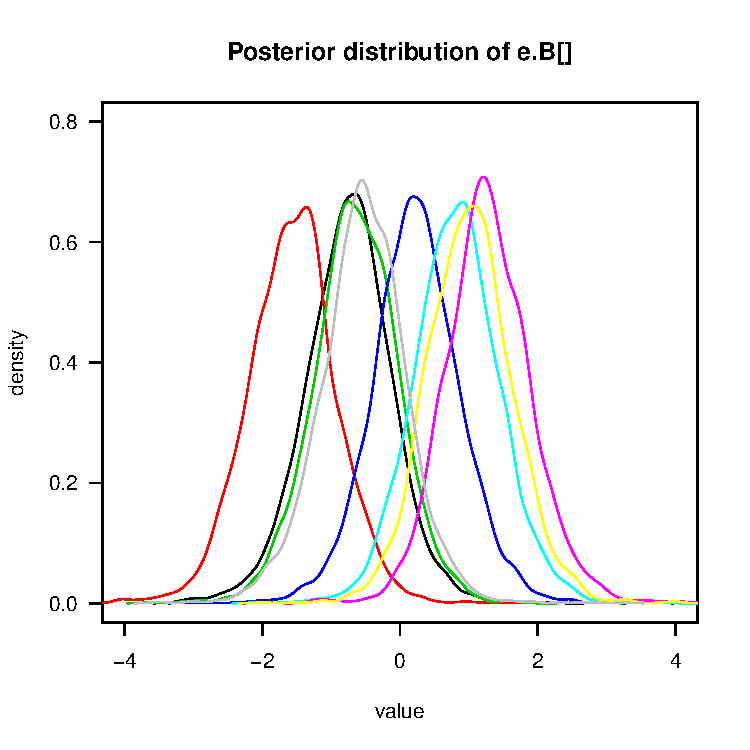
\includegraphics[bb=0 0 360 360, clip, width=270 bp]{example3_e.pdf}
	\end{center}
	\caption{\texttt{e.B[]}の事後分布}
	\label{example3_e_plot}
\end{figure}

%ページ調整
%\pagebreak

\subsubsection*{Nested Indexing}
上の例では2次元配列を使用しているが,配列のインデックスに配列を使用
するNested Indexingという方法もあるので,その例も紹介する。
%データファイルは同じく``\texttt{example3.csv}''だが,
 %\textsf{R}スクリプトは``\texttt{example3-1.R}'',
BUGS言語によるモデルは``\texttt{example3-1\_model.txt}''である。

\paragraph{データ}

まずデータを読み込む。このとき,
データを行列にはせず,ベクトルのままとする。
\begin{lstlisting}
> data <- read.csv("example3.csv")
> n.block <- 8           # number of blocks
> n.row <- nrow(data)    # number of observations
\end{lstlisting}

\texttt{data\$block}にどのブロックのデータであるかが格納されている。
\begin{lstlisting}
> data$block
 [1] 1 1 1 1 1 2 2 2 2 2 3 3 3 3 3 4 4 4 4 4 5 5 5 5 5 6
[27] 6 6 6 6 7 7 7 7 7 8 8 8 8 8
\end{lstlisting}

\paragraph{モデル}

モデルは以下のようになる。\texttt{X1},\texttt{X2},\texttt{Y}が1次元配列に
なっているところ(4〜5行目),\texttt{B}という変数が導入されているところ(6行目),
\texttt{e.B}のインデキシングが\texttt{B}を間に挟んでいるところ(16行目)などが
前のモデルと異なっている。

\begin{lstlisting}
var
  M,                    # Number of blocks
  N,                    # Number of observations
  X1[N], X2[N],         # Data
  Y[N],
  B[N],                 # Block
  e.B[M],               # Random effect
  beta, beta.1, beta.2, # Parameters
  tau, sigma,
  tau.B, sigma.B;       # Hyperparameters

model {
  # Likelihood
  for (i in 1:N) {
    Y[i] ~ dnorm(mu[i], tau)
    mu[i] <- beta + beta.1 * X1[i] +
                    beta.2 * X2[i] + e.B[B[i]]
  }
  for (i in 1:M) {
    e.B[i] ~ dnorm(0, tau.B)
  }

  # Priors
  beta ~ dnorm(0, 1.0E-4)
  beta.1 ~ dnorm(0, 1.0E-4)
  beta.2 ~ dnorm(0, 1.0E-4)
  tau <- 1 / (sigma * sigma)
  tau.B <- 1 / (sigma.B * sigma.B)
  sigma ~ dunif(0, 1.0E+4)
  sigma.B ~ dunif(0, 1.0E+4)
}
\end{lstlisting}

\paragraph{実行}

\texttt{jags.model()}関数の\texttt{data}引数は以下のようにする。
\begin{lstlisting}
model <- jags.model(file = model.file,
                    data = list(M = n.block, N = n.data,
                                X1 = data$x1, X2 = data$x2,
                                Y = data$y, B = data$block),
                    inits = inits, n.chains = n.chains,
                    n.adapt = 1000)
\end{lstlisting}

この方法は,前のモデリング方法とは異なり,ブロックごとにデータの数が違うときにも使える。

\subsubsection*{中央化(centering)}

モデル中の説明変数には,それぞれの平均を引いた値をかわりに使用(centering)した
方がマルコフ連鎖の自己相関が小さくなる(参考文献\cite{McCarthy}のBox 5.8)。
たとえば前のモデルなら,15行目の\texttt{beta.1 * X1[i]}を
\texttt{beta.1 * (X1[i] - X1.bar)}とする(\texttt{X1.bar}は\texttt{X1}の平均)。

ただし,\textsf{JAGS}で\texttt{glm}モジュールを使用した場合にはこの技法は不要である
(JAGS User's Manual\cite{JAGS} 4.6節)。


%%
%% Zero-Inflated Poissonモデル
%%
\subsection{ゼロ過剰ポアソンモデル}
\label{path}

最後の例題として,実際のデータを解析してみる。

\paragraph{データ}
このデータは,銀閣寺山国有林(京都市左京区)において,クロバイという木の芽生えの数を調べたものである。
調査したのは2002年で,1m×1mの大きさの方形区36か所について,その中で発芽してきた芽生えの数を数えた。
また,各方形区において全天写真を撮影し,それをもとに林冠開空率を求めた。
芽生えの数と林冠開空率との間に関連性があるかどうかを検討する。

データは``\texttt{example4.csv}''というファイルに入っている。
\begin{lstlisting}
"Plot","Num","Light"
1,0,2.680
2,0,1.030
3,3,1.899
   :
36,1,0.412
\end{lstlisting}
\noindent
\texttt{Plot}は方形区番号,\texttt{Num}は芽生えの数,\texttt{Light}は林冠開空率(\%)である。
開空率と芽生えの発生数とをプロットしてみると,図\ref{example4_scatter}のようになる。

\begin{figure}[hbtp]
  \begin{center}
    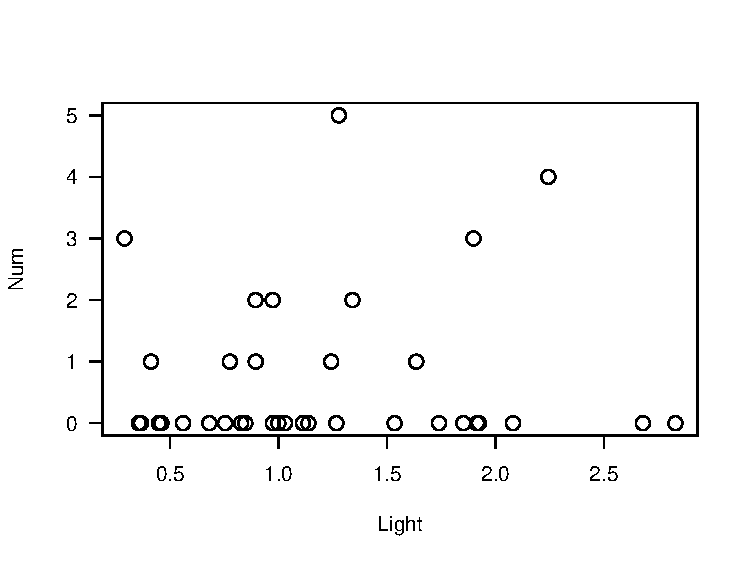
\includegraphics[bb=0 0 360 270, clip, width=300 bp]{example4_scatter.pdf}
  \end{center}
  \caption{開空率と芽生えの発生数との関係}
  \label{example4_scatter}
\end{figure}

単純に,誤差構造をポアソン分布(リンク関数をlog)とした一般化線形モデル(GLM)を適用すると,
以下のような結果となる。

\begin{lstlisting}
> summary(glm(Num ~ Light, family = poisson, data = data))

Call:
glm(formula = Num ~ Light, family = poisson, data = data)

Deviance Residuals: 
    Min       1Q   Median       3Q      Max  
-1.3831  -1.1942  -1.1473   0.3681   3.2771  

Coefficients:
            Estimate Std. Error z value Pr(>|z|)
(Intercept)  -0.5453     0.4234  -1.288    0.198
Light         0.1769     0.2929   0.604    0.546

(Dispersion parameter for poisson family taken to be 1)

    Null deviance: 65.608  on 35  degrees of freedom
Residual deviance: 65.252  on 34  degrees of freedom
AIC: 99.823

Number of Fisher Scoring iterations: 6
\end{lstlisting}

残差逸脱度(Residual deviance)の値が自由度(degree of freedom)の2倍程度となっている。
これは,過分散(overdispersion)が発生していることを示唆している。

もう一度,データをよくみてみると,芽生えの数に0が多いことがわかる(図\ref{example4_barplot})。
このような状態はゼロ過剰(Zero-inflated)と呼ばれる。
こうしたデータを扱うためには,ポアソン分布からはずれて0が多いことを,
そもそも存在する可能性がない場合があると考えて
モデル化する。
このようなモデルはゼロ過剰ポアソンモデル(Zero-Inflated Poisson model; ZIP model)と呼ばれる。

\begin{figure}[hbtp]
  \begin{center}
    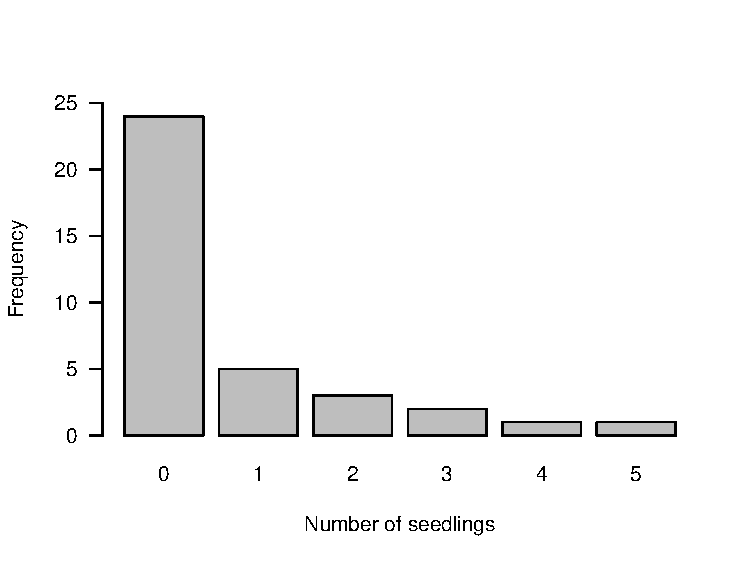
\includegraphics[bb=0 0 360 270, clip, width=300 bp]{example4_barplot.pdf}
  \end{center}
  \caption{芽生えの発生数の頻度分布}
  \label{example4_barplot}
\end{figure}

%ページ調整
%\vspace{2zw}

\paragraph{モデル}
ZIPモデルを扱うBUGSコードは以下のようになる。

\begin{lstlisting}
var
  N,         # Number of observations
  Y[N],      # Number of new seedlings
  X[N],      # Proportion of open canopy
  lambda[N], # Poisson mean
  z[N],      # 0: absent, 1: at least latently present
  p,         # Probability of the presence (at least latently)
  beta,      # Intercept in the linear model
  beta.x;    # Coefficient of X in the linear model
model {
  # Likelihood
  for (i in 1:N) {
    Y[i] ~ dpois(lambda[i])
    lambda[i] <- z[i] * exp(beta + beta.x * X[i])
    z[i] ~ dbern(p)
  }

  # Priors
  p ~ dunif(0, 1)
  beta ~ dnorm(0, 1.0E-4)
  beta.x ~ dnorm(0, 1.0E-4)
}
\end{lstlisting}

%% モデルの説明

芽生えの数が0となるのは以下の2通りであるとしてモデル化している。
\begin{enumerate}
\item 潜在的にも存在しない場合($z=0$)
\item 潜在的には存在する可能性があるが($z=1$)
ポアソン分布にしたがって0となった場合($\mathrm{Poisson}(0|\lambda)$)
\end{enumerate}
そして,$z$が0になるか1になるかは,確率$p$のベルヌーイ分布にしたがうとする。
潜在的には存在する可能性がある場合には,ポアソン分布部分の平均$\lambda$は
$\log\lambda = \beta + \beta_{x}X$であるとする。

\paragraph{結果}
これも同様に\textsf{rjags}を使って計算したところ
(burn-in 2000回,繰り返し回数 10000回,サンプリング間隔 10回),結果は以下のようになった。

\begin{lstlisting}
> summary(post)

Iterations = 2010:12000
Thinning interval = 10 
Number of chains = 3 
Sample size per chain = 1000 

1. Empirical mean and standard deviation for each variable,
   plus standard error of the mean:

          Mean     SD Naive SE Time-series SE
beta   -0.1031 0.5936 0.010837       0.018007
beta.x  0.5063 0.4172 0.007617       0.012891
p       0.4328 0.1050 0.001917       0.001985

2. Quantiles for each variable:

          2.5%     25%      50%    75%  97.5%
beta   -1.3386 -0.4852 -0.08479 0.3170 1.0068
beta.x -0.3120  0.2206  0.50906 0.7882 1.3116
p       0.2432  0.3591  0.42538 0.5015 0.6552

\end{lstlisting}
存在する確率$p$の事後平均は0.431,95\%信用区間は0.247〜0.650と推定された。
また,線形モデル部分の切片$\beta$および開空率の係数$\beta_{x}$の事後平均はそれぞれ
-0.09および0.498と,95\%信用区間はそれぞれ-1.226〜1.017および-0.323〜1.249
と推定された。開空率の係数の事後平均は,GLMでの推定値0.177よりも大きい値と
なった。

%ページ調整
%\pagebreak

\section{さらに学ぶには}

今回紹介したモデルは,モデルとしては簡単なものである。
実際に研究で使用されるモデルはもっと複雑なものであることが多い。
``Models for Ecological Data''\cite{Clark},
``Hierarchical modelling for the environmental sciences''\cite{Clark_Gelfand},
``Introduction to WinBUGS for ecologists''\cite{IWE},
``Bayesian population analysis using WinBUGS''\cite{BPA},
``Bayesian methods for ecology''\cite{McCarthy}などにて,
生態学・環境科学における実例が紹介されている。

日本語のものでは,
『データ解析のための統計モデリング入門』\cite{Kubo:Modeling}が,
GLM$\rightarrow$GLMM$\rightarrow$階層ベイズモデル
と,順序を追ってわかりやすく説明している。
空間統計モデリングについては,2009年の『日本生態学会誌』において,
久保\cite{Kubo}がその基本を解説して
おり,深澤ほか\cite{Fukasawa_et_al}が実例の紹介をおこなっている。
『マルコフ連鎖モンテカルロ法』\cite{Toyoda}には,
共分散構造分析におけるベイズ推定など,社会科学への応用例がある。
また,『岩波データサイエンス Vol.1』\cite{Iwanami_vol1}には,
\textsf{JAGS}や\textsf{Stan}などを用いた解析方法の記事があり,
サポートページ\footnote{\url{https://sites.google.com/site/iwanamidatascience/vol1/support_tokushu}}では,
コードや解説動画なども公開されている。


その他,MCMCや階層ベイズモデルについて目に付いたものを参考文献リストに入れて
おいたので,参考にされたい。

%ページ調整
%\pagebreak

%% 参考文献
\begin{thebibliography}{99}
\bibitem{PRML} Bishop C.M. (2006) Pattern recognition and machine learning.
  Springer-Verlag, New York.
  (日本語訳: 元田浩・栗田多喜夫・樋口知之・松本裕治・村田昇監訳 (2012)
  「パターン認識と機械学習 上/下」丸善, 東京)
\bibitem{Handbook} Brooks S., Gelman A., Jones G.L., Meng X.-L. (2011)
Handbook of Markov chain Monte Carlo. Chapman \& Hall/CRC, Boca Raton. 
\bibitem{Clark} Clark J.S. (2007) Models for ecological data.
  Princeton University Press, Princeton.
\bibitem{Clark_Gelfand} Clark J.S., Gelfand A.E. (2006) Hierarchical modelling
  for the environmental sciences. Oxford University Press, New York.
%\bibitem{Fukasawa} 深澤圭太・角谷拓 (2009) 始めよう! ベイズ推定によるデータ解析.
%  日本生態学会誌 59:167--170.\\
%  \texttt{http://ci.nii.ac.jp/naid/110007340208}
\bibitem{Fukasawa_et_al} 深澤圭太・石濱史子・小熊宏之・武田知己・田中信行・
  竹中明夫 (2009) 条件付き自己回帰モデルによる空間自己相関を考慮した生物の分布
  データ解析. 日本生態学会誌 59:171--186. \\
  \url{http://ci.nii.ac.jp/naid/110007340206}
\bibitem{Furutani} 古谷知之 (2008) ベイズ統計データ分析 --- R \& WinBUGS ---.
  朝倉出版, 東京.
\bibitem{BDA3} Gelman A, Carlin J.B., Stern H.S., Dunson D.B., Vehtari A.,
  Rubin D.B. (2014) Bayesian data analysis, 3rd ed.
  Chapman \& Hall/CRC, Boca Raton.
\bibitem{Gilks} Gilks W.R., Richardson S.R., Spiegelhalter D.J. (eds.) (1996)
  Markov chain Monte Carlo in practice. Chapman \& Hall/CRC, Boca Raton.
\bibitem{Iba} 伊庭幸人 (2003) ベイズ統計と統計物理. 岩波書店, 東京.
\bibitem{Iba2005} 伊庭幸人 (2005) マルコフ連鎖モンテカルロ法の基礎. 
  (伊庭幸人・種村正美・大森裕浩・和合肇・佐藤整尚・高橋明彦(著)
  「計算統計II ---マルコフ連鎖モンテカルロ法とその周辺---」
  岩波書店, 東京): 1--106.
\bibitem{Iwanami_vol1} 岩波データサイエンス刊行委員会(編) (2015) 岩波データサイエンス Vol.1.
岩波書店, 東京. \\
シリーズサポートページ \url{https://sites.google.com/site/iwanamidatascience/}
\bibitem{IWE} K\'ery M. (2010) Introduction to WinBUGS for ecologists:
  a Bayesian approach to regression, ANOVA, mixed models and related analyais.
  Academic Press, Waltham.
\bibitem{BPA} K\'ery M., Schaub M. (2011) Bayesian population analysis using WinBUGS --- A hierarchical perspective.
  Academic Press, Waltham.
    (日本語訳: 飯島勇人・伊東宏樹・深谷肇一・正木隆訳 (2016) 「BUGSで学ぶ階層モデリング入門---個体群のベイズ解析---」共立出版, 東京.)
\bibitem{Kery2015} K\'ery M., Royle J.A. (2015) Applied Hierarchical Modeling in Ecology --- Analysis of distribution, abundance and species richness in R and BUGS, Volume 1. Academic Press, Waltham.
\bibitem{DBDA2} Kruschke J. (2014) Doing Bayesian data analysis, 2nd ed.:
  a tutorial with R, JAGS, and Stan. Academic Press, Waltham.
\bibitem{Kubo} 久保拓弥 (2009) 簡単な例題で理解する空間統計モデル. 
  日本生態学会誌 59: 187--196. \\
  \url{http://ci.nii.ac.jp/naid/110007340204}
\bibitem{Kubo:IEICE} 久保拓弥 (2009) 最近のベイズ理論の進展と応用[I]
  階層ベイズモデルの基礎. 電子情報通信学会誌 92:881--885.\\
  \url{http://eprints.lib.hokudai.ac.jp/dspace/handle/2115/39717}
\bibitem{Kubo:Modeling} 久保拓弥 (2012) データ解析のための統計モデリング入門 ---
   一般化線形モデル・階層ベイズモデル・MCMC---. 岩波書店, 東京.
\bibitem{Kyo} 姜興起 (2010) ベイズ統計データ解析. 共立出版, 東京.
\bibitem{Link2012} Link, W.A., Eaton, M.J. (2012) On thinning of chains in MCMC.
Methods in Ecology and Evolution 3: 112--115. doi: 10.1111/j.2041-210X.2011.00131.x
\bibitem{OpenBUGS} Lunn D., Spiegelhalter D., Thomas A., Best N. (2009)
  {The BUGS project: Evolution, critique, and future directions}.
  {Statistics in Medicine} {28}:3049--3067.
\bibitem{BUGSBook} Lunn D., Jackson C, Besk N., Thomas A., Spiegelhalter D.
  (2012) The {BUGS} Book. Chapman \& Hall/CRC, Boca Raton.
\bibitem{MCMCpack} Martin A.D., Quinn, K.M. (2006) Applied Bayesian inference in R
using MCMCpack. R News 6(1):2--7. \\
    \url{http://cran.r-project.org/doc/Rnews/Rnews_2006-1.pdf}
%\bibitem{Martin} Martin J-M, Robert C. P. (2007) Bayesian core: A practical
%  approach to computational Bayesian statistics. Springer, New York.
\bibitem{McCarthy} McCarthy M.A. (2007) Bayesian methods for ecology.
  Cambridge University Press, New York.
  (日本語訳: 野間口眞太郎訳 (2009) 「生態学のためのベイズ法」共立出版, 東京.)
\bibitem{Ntzoufras} Ntzoufras I. (2009) Bayesian modeling using WinBUGS.
  Wiley, Hoboken.
\bibitem{JAGS} Plummer M. (2017) JAGS version 4.3.0 user manual.\\
  \url{http://sourceforge.net/projects/mcmc-jags/}
\bibitem{R} R Core Team (2017)
   R: A Language and Environment for Statistical Computing.
   R Foundation for Statistical Computing, Vienna.\\
   \url{http://www.R-project.org/}
\bibitem{IMCMR} Robert C.P., Casella G. (2010) Introducing Monte Carlo Methods with R.
  Springer, New York.
  (日本語訳: 石田基広・石田和枝訳 (2012) 「Rによるモンテカルロ法入門」丸善, 東京.)
\bibitem{WinBUGS} Spiegelhalter D., Tomas A., Best N., Lunn D. (2003)
  WinBUGS user manual version 1.4.\\
  \url{http://www.mrc-bsu.cam.ac.uk/bugs/winbugs/manual14.pdf}
\bibitem{Stan} Stan Development Team (2017) Stan Modeling Language:
  User's Guide and Reference Manual, Version 2.16.0.
  \url{http://mc-stan.org/}
\bibitem{Tango} 丹後俊郎 (2000) 統計モデル入門. 朝倉書店, 東京.
\bibitem{Terui} 照井伸彦 (2010) Rによるベイズ統計分析. 朝倉書店, 東京.
\bibitem{BUGS} Thomas A. (2006) The BUGS language.
  R News 6(1): 17--21. \\
  \url{http://cran.r-project.org/doc/Rnews/Rnews_2006-1.pdf}
\bibitem{Thomas} Thomas A., O'Hara B., Ligges U., Sturtz S. (2006) Making BUGS open.
  R News 6(1): 12--17. \\
  \url{http://cran.r-project.org/doc/Rnews/Rnews_2006-1.pdf}
%\bibitem{Tomita} 富田基史・花岡創 (2009) 階層ベイズモデルによる複雑な生態学的
%  プロセスの推定: ブナの花粉散布空間パターン推定を例に.
%  日本生態学会誌 59: 197--206.  \\
%  \texttt{http://ci.nii.ac.jp/naid/110007340202}
\bibitem{Toyoda} 豊田秀樹 (2008) マルコフ連鎖モンテカルロ法. 朝倉書店, 東京.
\bibitem{Toyoda2015} 豊田秀樹(編著) (2015) 基礎からのベイズ統計学
  ---ハミルトニアンモンテカルロ法による実践的入門---. 朝倉書店, 東京.
\bibitem{Wagou} 和合肇 (2005) ベイズ統計学による分析. (牧厚志・和合肇・
  西山茂・人見光太郎・吉川肇子・吉田栄介・濱岡豊(著)「経済・経営のための
  統計学」有斐閣, 東京):243--284.
\bibitem{Watanabe} 渡辺澄夫 (2012) ベイズ統計の理論と方法. コロナ社, 東京.
%\bibitem{Yamamichi} 山道真人・角谷拓 (2009) マルコフ連鎖モンテカルロ(MCMC)法を
%  用いたシミュレーションモデルのパラメータ推定: ベイジアンキャリブレーション入門.
%  日本生態学会誌 59:207--216. \\
%  \texttt{http://ci.nii.ac.jp/naid/110007340200}
\end{thebibliography}


\end{document}
